\documentclass[11pt,a4paper,serbian,oneside]{book}
\usepackage[utf8x]{inputenc}
\usepackage[T2A]{fontenc}
\usepackage{amsmath}
\usepackage{amssymb}
\usepackage{textcomp}
\usepackage{amsfonts}
\usepackage{graphicx}
\usepackage{ucs}
\usepackage{listings}
\usepackage[serbianc]{babel}
\usepackage{pdfsync}
\usepackage[left=2.5cm,right=2.5cm,top=2.5cm,bottom=2.5cm]{geometry}
\usepackage{float}

% Komanda za horizontal ruler
\newcommand{\HRule}{\rule{\linewidth}{0.5mm}}

%
% Definicija fiksiranih reci
%
\addto\captionsserbian{%
 \def\prefacename{Предговор}%
 \def\refname{Списак литературе}%
 \def\abstractname{Сажетак}%
 \def\bibname{Литература}%
 \def\chaptername{Глава}%
 \def\appendixname{Додатак}%
 \def\contentsname{Садржај}%
 \def\listfigurename{Списак слика}%
 \def\listtablename{Списак табела}%
 \def\indexname{Регистар}%
 \def\figurename{Слика}%
 \def\tablename{Табела}%
 \def\partname{Део}%
 \def\enclname{Прилози}%
 \def\ccname{Копије}%
 \def\headtoname{Прима}%
 \def\pagename{Страна}%
 \def\seename{Види}%
 \def\alsoname{Види такође}%
 \def\proofname{Доказ}%
 \def\glossaryname{Речник непознатих речи}
 \def\contentsname{Садржај}%
 }%

%
% Podesavanja paketa za listinge
%
\renewcommand\lstlistingname{Листинг}
\lstset {
	basicstyle=\footnotesize\ttfamily,
	numbers=left,
	numberstyle=\tiny,
	%stepnumber=2,
	numbersep=5pt,
	tabsize=2,
	extendedchars=true,
	breaklines=true,
	keywordstyle=\color{blue},
	frame=b,
	stringstyle=\color{green!50!black}\ttfamily,
	showspaces=false,
	showtabs=false,
	xleftmargin=17pt,
	framexleftmargin=14pt,
	framexrightmargin=3pt,
	framexbottommargin=4pt,
	framextopmargin=0pt,
	%backgroundcolor=\color{lightgray},
	showstringspaces=false,
   commentstyle=\color{green!50!black},
}

\lstloadlanguages {
	% Check Documentation for further languages ...
	%[Visual]Basic
	%Pascal
	C,
    C++,
	%Java,
	XML
	%HTML
}

%
% Podesavanje okvira listinga
%
\usepackage{color}
\usepackage{xcolor}
\usepackage{caption}
\DeclareCaptionFont{white}{\color{white}}
\DeclareCaptionFormat{listing}{\colorbox[cmyk]{0.43, 0.35, 0.35,0.01}{\parbox{\textwidth}{\hspace{12pt}#1#2#3}}}
\captionsetup[lstlisting]{format=listing,labelfont=white,textfont=white, singlelinecheck=false, margin=0pt, font={bf,footnotesize} }

%
% Dupla kosa crta
%
\usepackage{stmaryrd}

%
% Pocetak dokumenta
%
\begin{document}

%
% Naslovna stranica
%

\begin{titlepage}

\begin{center}

% Gornji deo stranice

\includegraphics[width=0.25\textwidth]{logo-pmf.pdf}\\[1cm]    

\textsc{\LARGE Институт за математику и информатику
\\ Природно-математички факултет
\\ Универзитет у Крагујевцу}\\[1.5cm]

\textsc{\Large Мастер рад}\\[0.5cm]

% Naslov
\HRule \\[0.4cm]
{ \huge \bfseries Примена алгоритама препознавања облика у неутронској дозиметрији}\\[0.4cm]

\HRule \\[1.5cm]

% Autor i mentor
\begin{minipage}{0.4\textwidth}
\begin{flushleft} \large
\emph{Студент:}\\
Никола Николић
\end{flushleft}
\end{minipage}
\begin{minipage}{0.4\textwidth}
\begin{flushright} \large
\emph{Професор:} \\
др Милош Ивановић
\end{flushright}
\end{minipage}

\vfill

% Dno stranice
{\large Септембар 2014.}

\end{center}

\end{titlepage}


%%%%%%%%%%%%%%%%%%%%%%%%%%%%%%%%
%
% Поглавље:
%
% Садржај
%
%%%%%%%%%%%%%%%%%%%%%%%%%%%%%%%%

\tableofcontents
\newpage

%%%%%%%%%%%%%%%%%%%%%%%%%%%%%%%%
%
% Поглавље:
%
% Сажетак
%
%%%%%%%%%%%%%%%%%%%%%%%%%%%%%%%%

\chapter*{Сажетак}

Дозиметрија се бави одређивањем апсорбоване дозе јонизујућег зрачења у разним ма\-те\-ри\-ја\-ли\-ма, укључујући и људско ткиво. Карактеристике тренутно доступних личних неуторнских дозиметара су далеко од идеалних, а траг детектори се данас сматрају једном од најперспективнијих техника. Међу њима је најпознатији \textit{CR-39} детектор. При ин\-те\-рак\-ци\-ји упадних неутрона са детектором настају трагови који нагризањем материјала базом постају видљиви. На основу тих трагова врши се процена дозе зрачења. 

Мерење густине трагова врши се визуелном проценом броја трагова по јединици по\-вр\-ши\-не помоћу микроскопа. Тај процес може да траје и по више сати. У овом раду ће се описати примена алгоритама обраде слика (\textit{image processing}) која овај процес може делимичнио аутоматизовати и значајно убрзати.

У првом поглављу дат је увод у неутронску дозиметрију, њену примену и дефинисан је проблем којим ће се бавити овај рад. Друго поглавље представља \textit{OpenCV} библиотеку и описује коришћене алгоритме за обраду слика. Треће поглавње укратко представља \textit{Qt} платформу за развој корисничког интерфејса и његове главне предности. У четвртом поглављу описан је софтвер за детекцију трагова неутронске дозиметрије. Дат је опис структуре пројекта као и начин употребе развијеног софтвера. Даље, у петом поглавњу дата је анализа софтвера, процена тачности детекције трагова, као и анализа најчешћих грешака детекције. У последњем поглављу дат је предлог могућих унапређења апликације.

%%%%%%%%%%%%%%%%%%%%%%%%%%%%%%%%
%
% Поглавље 1:
%
% Увод у неутронску дозимертију
%
%%%%%%%%%%%%%%%%%%%%%%%%%%%%%%%%

\chapter{Увод у неутронску дозимертију}

\section{Атоми и зрачење}

Атом је основна јединица материје. Атоми су изграђени од позитивно наелектрисаног атомског језгра и одређеног броја електрона. Електрони носе негатвно наелектрисање и крећу се у електронском омотачу око језгра. Атомско језгро садржи протоне, који имају позитивно наелектрисање, једнако негативном наелектрисању електрона и неутроне који немају наелектрисање. 

\begin{figure}[h]
\begin{center}
\leavevmode
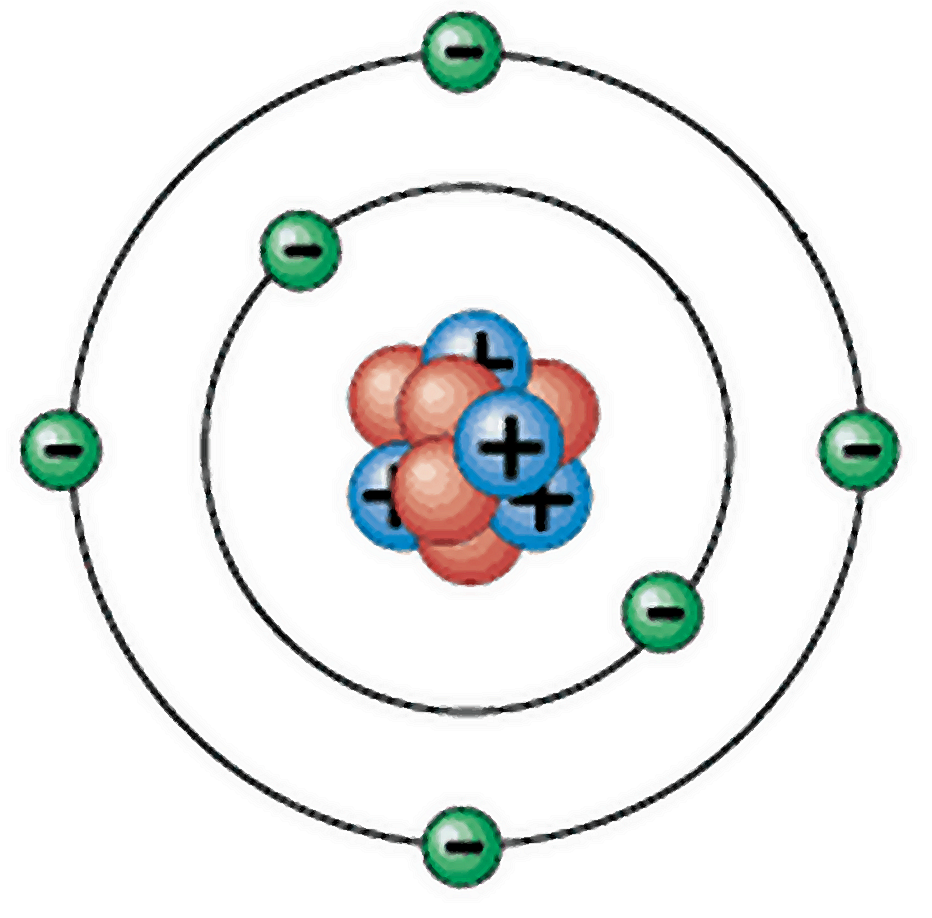
\includegraphics[width=50mm]{images/atom.png}
\end{center}
\caption{Шематски приказ структуре атома}
\label{fig:atom}
\end{figure}

Хемијске особине атома одређује број протона у језгру. Сваки атом садржи једнак број протона и електрона и зато је електрично неутралан.  Атом постаје наелектрисан тако што прими или отпусти један или више електрона и постаје јон. Такав процес назива се јонизација.

Како хемијске особине атома не зависе од броја неутрона, постоје атоми истог елемента са различитим бројем неутрона - тзв. изотопи. Атомска језгра са неповољним односом броја протона и броја неутрона су нестабилна и путем радиоактивног распада прелазе у стабилније стање.

Радиоактивност је спонтани процес у којем се атомско језгро, емитујући једну или више честица преображава у друго језгро. При трансформацији језгра, мења се састав или енергетско стање. Радиоактивно зрачење продире кроз различите материјале, а такође може и да јонизује средину кроз коју пролази. На тај начин може да изазове оштећење ћелија живих организама. Настали јони нарушавају биохемијске процесе у ћелијама, што може довести до разних поремећаја у њиховом функционисању и деоби, па и до настанка озбиљних болести.

\subsection{Типови зрачења}

Према ефектима које производи на материју, зрачење се може класификовати на јо\-ни\-зу\-ју\-ће и нејонизујуће зрачење.

Јонизујуће зрачење укључује космичке зраке, \textit{X} зраке и зрачење од радиоактивних материјала. Заједничко својство је висока енергија која омогућава јонизацију атома средине кроз коју зрачење пролази. Како долази до јонизације атома и молекула који су до тада били неутрални, настају оштећења материјала. Јонизирајуће зрачење спада у најопасније, оно је за око невидљиво, не осећа се код контаминације, тешко се детектује и постоји јако узак број терапија које могу помоћи. Три основна типа јонизујућег зрачења су $\alpha$, $\beta$ и $\gamma$ зрачење.

Нејонизујуће зрачење укључује ултраљубичасто светло, топлотно зрачење, радио таласе и слично. Не поседује енергију као јонизујуће зрачење и обично се сматра безопасним при малим дозама које не изазивају пораст температуре.

\begin{figure}[h]
\begin{center}
\leavevmode
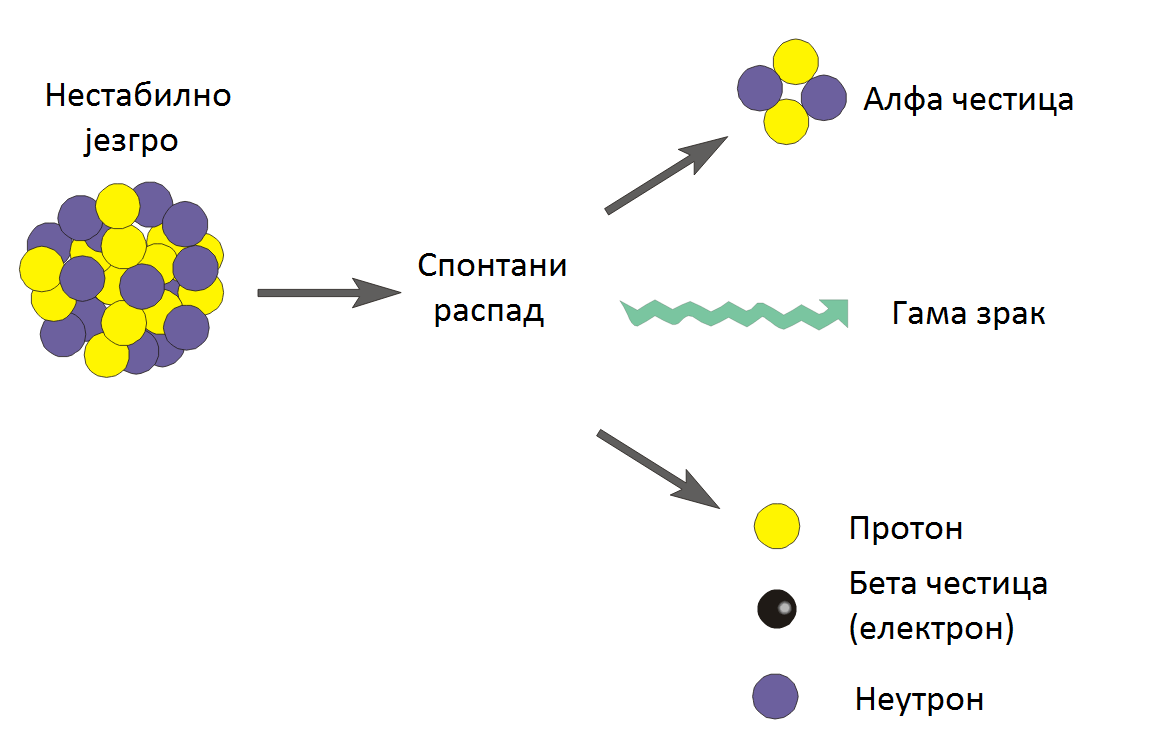
\includegraphics[width=120mm]{images/radiation.png}
\end{center}
\caption{Честице које могу настати при радиоактивном распаду}
%\label{fig:atom}
\end{figure}

\begin{itemize}

  \item \textbf{Алфа зрачење ($\alpha$)}. Алфа честица је позитивно наелектрисано језгро хелијума (језгро са два протона и два неутрона) емитовано од стране нестабилног атомског језгра. Алфа честица је релативно масивна, али има кратак домет у ваздуху, свега 3-5 \textit{cm}. Алфа честице могу апсорбовати кожа или папир.

  \item \textbf{Бета зрачење ($\beta$)}. Бета честице су вискоенергетски електрони или позитрони. Електрони настају распадом језгра са вишком неутрона, а позитрони настају при распаду језгра са вишком протона у односу на њихов оптимални број за стабилност језгра. Бета честице су много мање од $\alpha$ честица и могу продрети даље у материјал или ткиво. Бета зрачење се може апсорбовати материјалима од пластике, стакла или метала.
  
  \item \textbf{Гама зрачење ($\gamma$)} је врло високи енергетски фотон (форма електромагнетне ра\-ди\-ја\-ци\-је врло кратке таласне дужине), емитован од стране нестабилног језгра које често у исто време емитује и $\alpha$ и $\beta$ честице. Гама зрачење узрокује јонизацију у атомима када пролази кроз материјал, првенствено због интеракције са електронима. У одсуству густих материјала, $\gamma$ зрачење може оштетити материјал на који делује.

  \item \textbf{Неутронско зрачење (\textit{n})} је емитовање неутрона из нестабилног језгра. Ван језгра неутрони су нестабилни и имају време полураспада око 11,5 минута. Када су у реакцији са материјалом изазивају емисију $\beta$ и $\gamma$ зрачења. Неутронско зрачење захтева значајну заштиту да би се редуковало излагање.

\end{itemize}

\subsection{Извори, примена и ефекти зрачења}

Изворе зрачења делимо на \textbf{природне} и \textbf{вештачке}. Природном зрачењу изложени смо услед зрачење Сунца и космоса, радиоактивних елемената у тлу, објектима у којима живимо, преко хране и пића које уносимо у тело. Количина овог неизбежног природног зрачења се разликује од места до места на Земљи.

Ефекти зрачења на људско здравље од природних извора нису изразито негативни, јер се оно никад не сакупља у телу. Природно зрачење је стално и веома слабо. Биолошки механизам је еволутивно прилагођен на ову врсту зрачења.

Вештачки извори радијације на Земљи премашују 5\% укупног зрачења. Ови извори зрачења су они које је човек изградио: 

\begin{itemize}

  \item \textbf{Нуклеарне електране} имају за циљ да произведу електричну енергију. Највећу и сталну потецијалну опасност у раду нуклеарних електрана чине евентуални инциденти при којима се емитују велике количине радиоактивног материјала у атмосферу и земљиште.

  \item \textbf{Медицински извори} зрачења настају при лечењу неких болести услед употребе апарата који емитују радиоактивно зрачење. Такође, истрошени апарати и опрема остају као проблем у виду радиоактивног отпада.

  \item \textbf{Технички извори} зрачења се односе на разне апарате који функционишу на бази радионуклеида, те представљају опасност за животну средину (радиоактивни гро\-мо\-бра\-ни, разни апарати у научно-истраживачким иституцијама).

\end{itemize}

Јонизујуће зрачење делује штетно на биолошке системе и може да доведе до појаве функционалних, морфолошких и генетских промена, а уколико су дозе којима је особа изложена високе може да дође и до смрти. Нису сви људи подједнако осетљиви на зрачење, као ни сва ткива и органи у организму.

Акутни ефекти се јављају непосредно после озрачивања особе код изложености високим дозама радијације. Јачина ефекта зависи од примљене дозе, врсте зрачења и осетљивости озрачених ткива. Код акутне озрачености јавља се радијациона болест.

Код хроничне изложености радиоактивном зрачењу, обично код професионално из\-ло\-же\-них особа, долази до оштећења ткива, и то најчешће крви и хематопоетских органа.  Уколико  се реагује на време, најчешће долази до опоравка. 

\section{Неутронско зрачење}

Неутрони су ненаелектрисани и не интереагују са електронима, па могу да прођу знатно растојање у материји без икакве интеракције. Понашање неутрона је слично $\gamma$ зрачењу, и оно припада групи индиректно јонизујућих зрачења. Међутим, неутрони не могу директно да јонизују материју, већ то чине искључиво преко секундарно произведених честица. 

Електромагнетска интеракција неутрона са електронима је занемарљива. Са друге стране, пролазећи кроз материју, неутрони се могу расејати еластично или нееластично на атомским језгрима. Расејање је еластично ако се укупна кинетичка енергија у судару очува, тј. када је енергија коју неутрон изгуби једнака кинетичкој енергији узмака језгра. Расејање је нееластично када језгро апсорбује извесну количину енергије и пређе у више енергетско стање. Такође, неутрон може бити захваћен или апсорбован од стране језгра, што доводи до промене броја неутрона захваћеног језгра, па самим тим и његових физичких и хемијских својстава.

За брзе неутроне је типично да највише губе енергију у материји преко еластичних расејања. Овај процес се назива модерација неутрона и један је од најважнијих процеса у нуклеарним реакторима. Како енергија неутрона опада, расејање се наставља, али ге\-не\-рал\-но, расте вероватноћа захвата на језгру. Дифузија термалних неутрона је такође узрокована низом еластичних расејања.

Еластично расејање неутрона се доста користи за регистровање брзих неутрона, про\-уча\-ва\-ју\-ћи узмакнута језгра (углавном узмакнуте протоне) различитим инструментима. Овај тип расејања се такође користи за регистровање узмакнутих језгара помоћу јонизационих метода.

\subsection{Примена неутронског зрачења}

Најважније примене неутронских извора су заступљене у индустрији, у науци и ис\-тра\-жи\-ва\-њу, као и у медицини:

\begin{itemize}
  
  \item \textbf{Геофизичка мерења}: мапирање и анализа рудника минерала, нафтна истраживања, мапирање и анализа каменолома, истраживање урана.

  \item \textbf{Контрола индустријских процеса}: контрола цементног процеса, испитивање ква\-ли\-те\-та угља, испитивање дебљине зида.

  \item \textbf{Медицина}: мерење састава тела, терапија канцера, студије дијете и исхране.

  \item \textbf{Безбедност}: детекција и идентификација експлозива, детекција и идентификација хемијског оружија, детекција и идентификација специјалних нуклеарних материјала, детекција нагазних мина.

  \item \textbf{Општа истраживања}: референтни извор брзих неутрона за инструментацију, ка\-ли\-бра\-ци\-они извор за инструментацију за посматрање нeутрина, проучавање осетљивости електронских компоненти на радијацију, испитивање нуклеарног реактора, неутронска радиографија.

  \item \textbf{Екологија}: испитивање нуклеарног отпада, испитивање отпада за очување ресурса и поступак опоравка, квантификација угљеника у земљишту.

\end{itemize}

\subsection{Дозиметрија}

Дозиметрија \cite{bmilenkovic} се бави одређивањем дозе јонизирајућег зрачења, првенствено у људском ткиву, али и у разним другим материјалима. Неутронска дозиметрија је од велике важности за заштиту од зрачења у близини акцелератора честица и нуклеарних реактора, за кван\-ти\-фи\-ка\-ци\-ју ефеката излагања космичком зрачењу, као и код терапије брзим и спорим неутронима.

Иако је развој нуклеарне физике и физике елементарних честица унео у употребу много врста детектора, они се заснивају на истом принципу: предаја дела или целокупне енергије зрачења детекторској маси, где се она преводи у неку другу форму енергије која је погодна за људско опажање.

За детекцију, неутралне честице најпре морају проћи кроз неку врсту реакције у де\-тек\-то\-ру, чији ће прозвод бити наелектрисане честице које јонизују или ексцитују атоме материјала детектора. Облик у коме се појављује енергија зависи од детектора и његове конструкције.  На пример, гасни детектори директно прикупљају јонизационе електроне за формирање струјног сигнала, док у сцинтилаторима  ексцитација и јонизација доприносе појави молекуларних прелаза, чији је крајњи резултат емисија светлости. У фотографским емулзијама, јонизација изазива хемијске реакције које омогућују формирање латентне слике трага.

Савремени детектори су претежно електричне природе. У неком тренутку, информација из детектора се претвара у електрични сигнал који је погодан за електронску обраду. Такви детектори користе активне методе за детекцију и дозиметрију неутрона. 

Поред активних, користе се и пасивне методе, односно методе које не захтевају директно напајање енергијом у току излагања.  Међу данас коришћеним пасивним личним не\-ут\-рон\-ским дозиметрима, траг детектори се сматрају једном од најперспективнијих техника. Посебно место у свету траг детектора заузима \textit{CR-39} детектор.

\subsubsection{\textit{CR-39} детектор}

Међу бројним предностима \textit{CR-39} детектора у односу на друге мерне технике су велика осетљивост на протоне, нискоенергетски праг за неутроне, као и неосетљивост на Гама зрачење. Због тога је \textit{CR-39} најпогоднији кандидат за примену у личној неутронској дозиметрији.

При расејању неутрона на атомима \textit{CR-39} детектора ($C_{12}H_{18}O_{7}$) производе се
узмакнута језгра H, C и O, док се у нуклеарним реакцијама стварају секундарне
наелектрисане честице ($\alpha$ честице, протони, деутерони...). Секундарне наелектрисане честице и узмакнута језгра остављају оштећења при проласку кроз детекторски материјал, која се називају "латентни трагови". Попречне димензије латентних трагова су до 10 nm, тако да се могу видети само под електронским микроскопом. Траг се може визуелизовати (учинити видљивим) под оптичким микроскопом, ако се делује агресивним хемијским агенсом, као што је на пример, водени раствор $NaOH$ или $KOH$. Услед веће хемијске активности, раствор нагриза оштећени део више него неоштећени, тако да се латентни траг знатно увећава и може се посматрати обичним оптичким микроскопом. Примери нагрижених трагова дати су на слици \ref{fig:trag}.

\begin{figure}[h]
\begin{center}
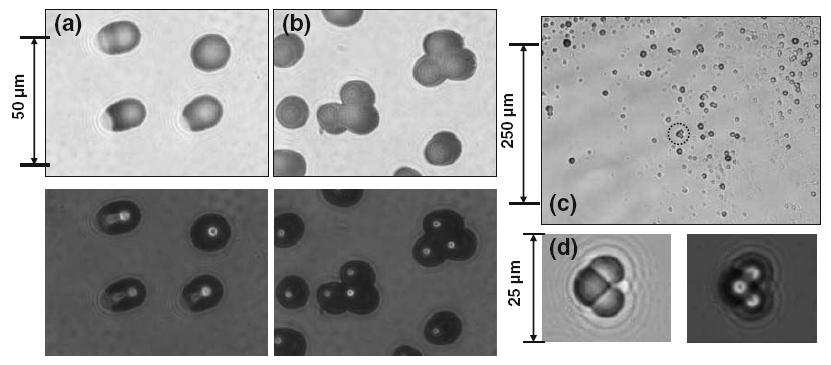
\includegraphics[width=150mm]{images/dosimetry.png}
\end{center}
\caption{Трагови настали озрачивањем \textit{CR-39} детектора}
\label{fig:trag}
\end{figure}

\section{Дефиниција проблема}

Mерење густине трагова насталих траг детектором \textit{CR-39} визуелном проценом броја трагова по јединици површине помоћу оптичког микроскопа траје незанемарљиво дуго. Још један од изазова је и опис развоја трага, односно раст трагова. Ови процеси могу да трају и по више сати. 

У складу са поменутим, основна хипотеза Мастер рада је да се овај посао може ауто\-ма\-ти\-зо\-ва\-ти и значајно убрзати применом алгоритама за обраду слика. Као основни програмерски алати користе се решења отвореног кода:
језик \textit{C++} спрегнут са библиотеком \textit{OpenCV (Open Source Computer Vision Library)}, као и \textit{Qt} платформа за израду корисничког ин\-тер\-феј\-са.

%%%%%%%%%%%%%%%%%%%%%%%%%%%%%%%%
%
% Поглавље 2:
%
% Обрада слика употребом OpenCV библиотеке
%
%%%%%%%%%%%%%%%%%%%%%%%%%%%%%%%%

\chapter{Обрада слика употребом библиотеке \textit{OpenCV}}

\textit{OpenCV (Open Source Computer Vision Library)} \cite{opencv} је библиотека отвореног кода, која садржи имплеметације више стотина алгоритама рачунарског вида (\textit{computer vision}). Би\-бли\-о\-те\-ка је написана у  програмском језику \textit{C++}, али подржава и итерфејсе ка програмским језицима \textit{C}, \textit{Python} и \textit{MATLAB}, а у развоју су и интерфејси за \textit{CUDA} и \textit{OpenCL} платформе. Подржана је на свим вoдећим оперативним системима: \textit{Windows}, \textit{Linux}, \textit{Android} и \textit{Mac OS X}. Библиотека је објављена под \textit{BSD} лиценцом, те је стога погодна  и за академску и за комерцијалну употребу.

Имплементирани алгоритми се могу користити за  препознавање облика, детекцију и препознавање лицa, праћење покрета при видео снимку, спајање више слика у једну, пре\-по\-зна\-ва\-ње маркера за проширену стварност и слично. Такви алгоритми су примењени у бројним реалним апликацијама, попут програма за видео надзор, навигацију и ауто\-ма\-ти\-за\-ци\-ју рада робота, проверу призвода у фабрикама, асистенцију при вожњи аутомобила итд.

Рачунарски вид помаже у прикупљању релевантних информација са слика и доношењу одлука базираних на тим подацима. Циљ рачунарског вида је да омогући да рачунар посматра ствари на исти начин као и људи. Основни кораци система базираног на ра\-чу\-нар\-ском виду су:

\begin{itemize} %\itemsep1pt \parskip0pt \parsep0pt
  \item прикуљање слика,
  \item манипулација сликама,
  \item извлачење релевантних информација и
  \item доношење одлука.
\end{itemize}

\begin{figure}[h]
\begin{center}
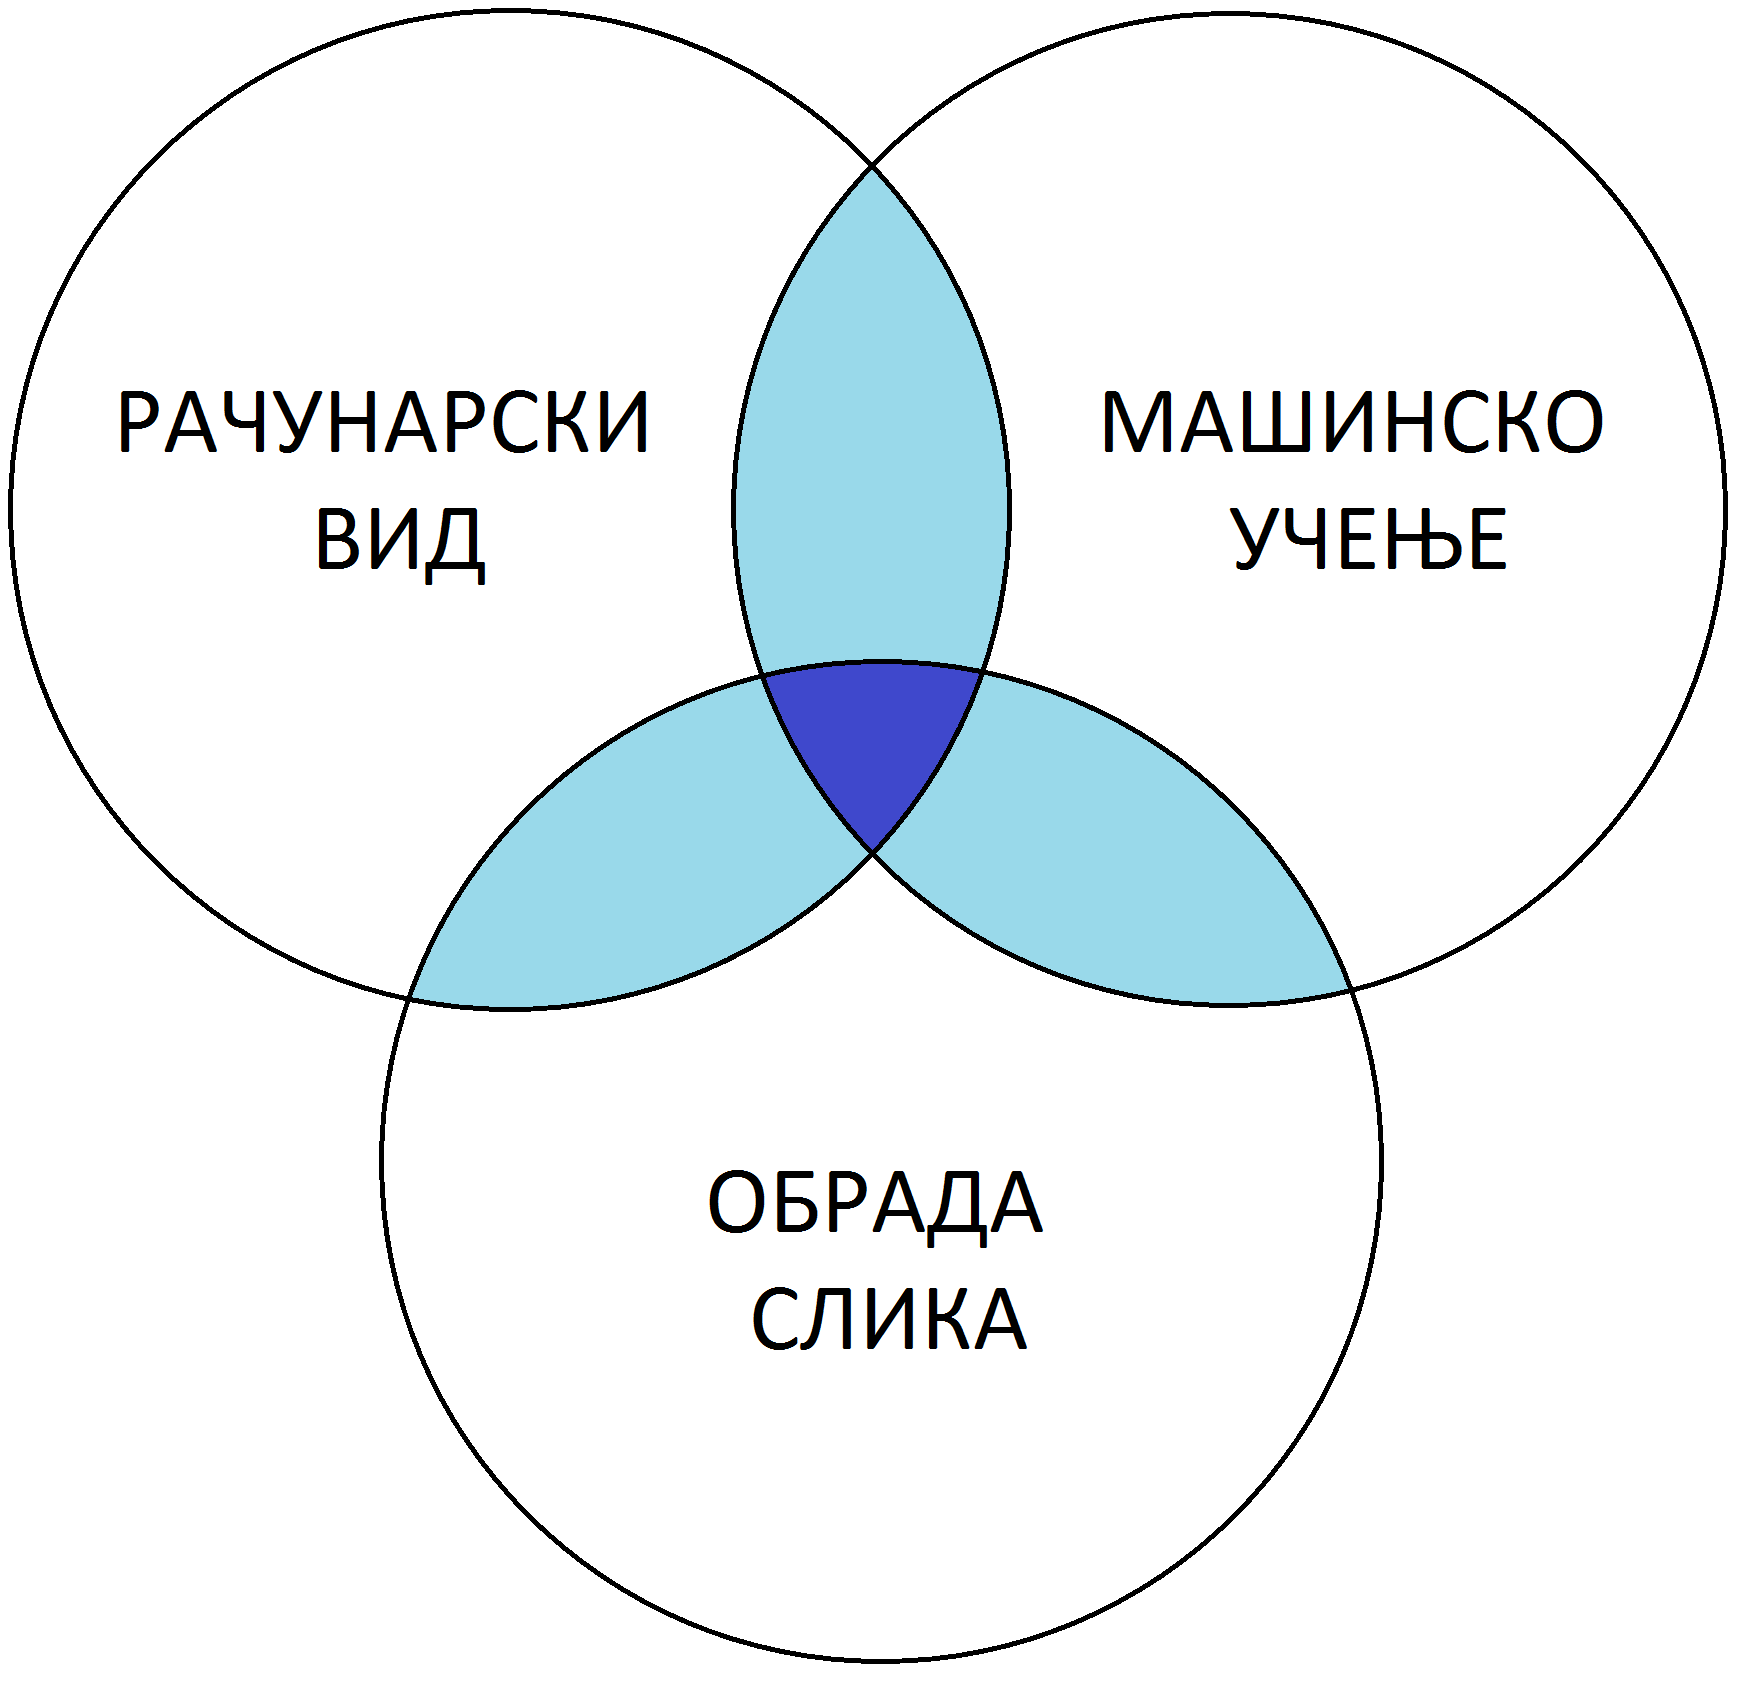
\includegraphics[width=75mm]{images/cv.png}
\end{center}
\caption{Однос рачунарског вида са машиснким учењем и обрадом слика}
\label{fig:cv}
\end{figure}

Као што се из наведеног види, за један такав систем веома су важни и алгоритми машинсог учења (\textit{machine learning}) као и алгоритми обраде слика (\textit{image processing}). Би\-бли\-о\-те\-ка \textit{OpenCV} садржи такве алгоритме. Компонента која нас занима је управо обрада слика. Обрада слика је процес манипулације подацима слике у сврху прикупљања ре\-ле\-ван\-тних информација. 

Софтвер, који је резултат овога рада, има задатак да са слике материјала неутронске дозиметрије изврши процену броја трагова зрачења. Кораци обраде слике и процене броја трагова дати су у наставку.

\section{Сиво скалирана слика}

Први корак за већину алгоритама обрадa слика је рачунање сиво скалиране слике на основу оригиналне слике, тј. слике која садржи црвену, зелену и плаву компоненту. У даљем процесу користи се само сиво скалирана слика. На тај начин  постиже се значајна уштеда у меморији, јер слика која се обрађује може бити интерно копирана више пута.  Самим тим постижу се боље перформансе, а добија се и на једноставности алгоритама.

\begin{lstlisting}[language=C++,label=lst:grayscale,caption=Рачунање сиво скалиране слике]
// Load BGR image.
Mat bgr = imread(path, CV_LOAD_IMAGE_COLOR);

// Convert image to grayscale.
Mat grayscale;
cvtColor(bgr, grayscale, CV_BGR2GRAY);
\end{lstlisting}

Сиво скалирана слика рачуна се као:
\begin{equation}
Y \gets 0.299 \cdot R + 0.587 \cdot G + 0.114 \cdot B,
\end{equation}
где су $Y$ - сиво скалирана слика, $R$ - црвена компонента оригиналне слике, $G$ - зелена компонента оригиналне слике и $B$ - плава компонента оригиналне слике. Коефицијенти представљају измерену перцепцију интензитета код трохроматских људи. Конкретно, људ\-ски вид је најосетљивији на зелену, а најмање на плаву боју.

\begin{figure}
\begin{center}
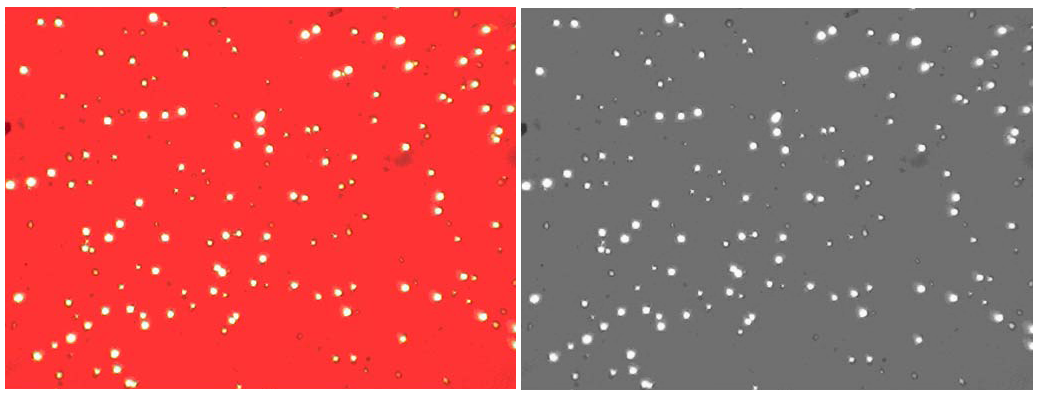
\includegraphics[width=150mm]{images/original+grayscale.png}
\end{center}
\caption{Оригинална (лево) и сиво скалирана (десно) слика}
\label{fig:cv}
\end{figure}

\newpage

\section{Сегментација слике}

Један од основних циљева обраде слика је идентификација објеката који се појављују на дигиталној слици. Задатак сегментације слике је да произведе поједностављене ин\-фор\-ма\-ци\-је за анализу. Сегментација пружа информације о позицији и изгледу објекта.

Постоје различите методе сегментације, а избор конкретне методе се врши на основу примене. Неке од најчешћих метода сегментације су:

\begin{itemize}

  \item \textbf{Сегментација прагом} (\textit{Thresholding}) - подрзумева раздвајање објеката на основу боје пиксела. У зависности од боје, пиксел припада одређеној групи објеката. Уколико се врши сегментација са једним прагом, метода се назива бинаризација. Бинаризација се најчешће користи за раздвајање објеката од позадине. Ово је најједноставнији и најбржи метод сегметације. Сегментација прагом се примељује у алгоритмима препознавања текста за раздвајање текста од позадине.

  \item \textbf{Сегметација кластеризацијом} (\textit{Clustering}) - подразумева груписање пиксела слич\-них карактеристика у групе/објекте. Поступак сегментације се састоји од рачунања вектора одлика за сваки пиксел, проналажења карактеристичних вектора пиксела (центара кластера који свакако припадају различитим објектима) и придруживање сваког пиксела једном од кластера. Ова метода се примењује са великим успехом у обради сателитских и авионских снимака, а највећа мана је велика рачунарска сложеност.
  
  \item \textbf{Детекција ивица} (\textit{Edge detection}) - подразумева проналажење тачака слике око којих се значајно мења интензитет боје. На овај начин добијају се линије које представљају ивице објеката. Пошто добијене линије нису увек спојене, додатно се користе алгортми за реконструкцију недостајућих сегмената. Детекција ивица је моћнији, али и спорији метод сегментације.
  
  \item \textbf{Слив} (\textit{Watershed}) - свака слика се може посматрати као топографска површина, где низак интензитет боје означава брда и врхове, а висок интензитет означава долине. Идеја алгоритма је да се свака изолована долина  (локални минимум интензитета боје) пуни различито обојеном водом. Са порастом нивоа, вода из различитих долина почиње да се спаја. Да би се избегло спајање, постављају се баријере на месту спајања.  Ниво воде наставља да расте све док сви врхови не буду под водом. Постављене баријере представљају резултат сегментације.

\end{itemize}
 
У сличају детекције трагова неутронске дозиметрије, трагови су јасно представљени и различитог су интензитета у односу на позадину. Могу бити представљени светлом бојом на тамној позадини или тамном бојом на светлој позадини. У сваком случају, издвајање трагова од позадине је релативно једноставан задатак. Компликованији случај је раздвајање трагова који се преклапају без јасне границе између преклопљених трагова. За решавање овог проблема користи се модификована верзија \textit{watershed} алгоритма. Основни кораци детекције трагова су:
\begin{enumerate}
  \item раздвајање трагова од позадине,
  \item проналажење трагова и
  \item сегментација трагова.
\end{enumerate}

У случају да су трагови превише преклопљени, сегметација трагова не може да их детектује као засебне трагове. Из тог разлога, оставља се могућност корекције трагова у каснијој процедури.

\subsection{Раздвајање трагова од позадине}

За раздвајање трагова од позадине користи се сегментација са једним прагом, односно бинаризација. Бинаризација подразумева раздвајање светлих и тамних делова слике, од\-нос\-но, у представљеном случају, идентификовање светлих објеката на тамној позадини.

\begin{figure}[htb]
\begin{center}
\leavevmode
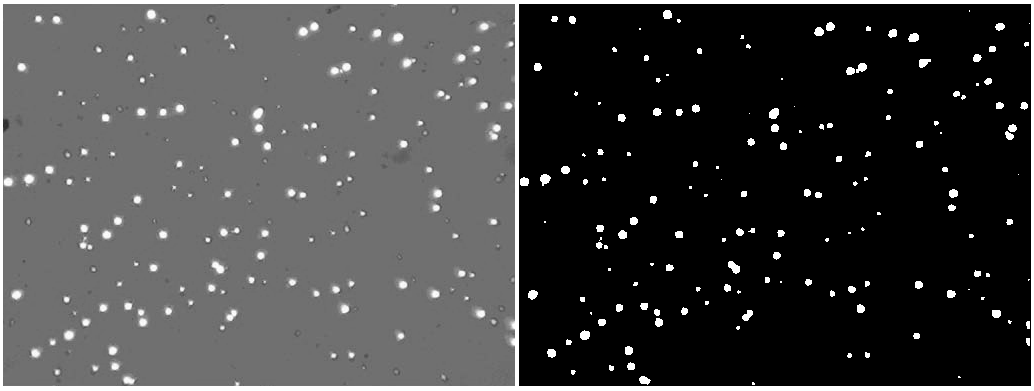
\includegraphics[width=150mm]{images/binary.png}
\end{center}
\caption{Сиво скалирана (лево) и бинарна/црно-бела (десно) слика}
\label{fig:cv}
\end{figure}

Улазни параметар за бинаризацију је сиво скалирана слика. Резултат бинаризације је црно-бела слика истих димензија као и сиво скалирана слика. Црна боја представља позадину, а белом бојом се означавају пиксели који припадају објектма. Вредност сваког пиксела резултујуће слике рачуна се као:
\begin{equation}
binary(x, y) = \left\{ 
  \begin{array}{l l}
    white, & \quad grayscale(x, y) > thresh,\\
    black, & \quad \text{иначе.}
  \end{array} \right.
\end{equation}
где је \textit{binary} - бинарна слика, \textit{grayscale} - сиво скалирана слика, \textit{thresh} - праг, \textit{white} - вредност белог пиксела, \textit{black} - вредност црног пиксела, а \textit{x} и \textit{y} одговарајући индекси пиксела слика.

\begin{lstlisting}[language=C++,label=lst:grayscale,caption=Рачунање бинарне слике са унапред задатим прагом]
// Calculate binary image.
threshold(
    grayscale, // Grayscale image.
    binary,    // Binary image.
    thresh,    // Threshold value.
    255,       // Max pixel value, i.e. white pixel walue.
    CV_THRESH_BINARY);
\end{lstlisting}

Праг према коме се врши класификација може бити и аутоматски одређена вредност помоћу \textit{Otsu} метода. Употребом овог метода креира се хистограм вредности пиксела. Према очекивању, постоје две класе вредности хистограма, и то једна за тамне пикселе и једна за светле пикселе. Као оптимална граница узима се средња вредност између те две класе.

\begin{figure}
\begin{center}
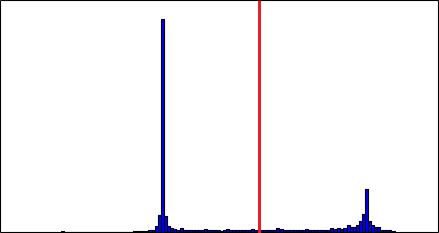
\includegraphics[width=100mm]{images/histogram.png}
\end{center}
\caption{Хистограм интензитета боје на сиво скалираној слици
и \textit{Otsu} праг}
\label{fig:otsu}
\end{figure}

 \begin{lstlisting}[language=C++,label=lst:grayscaleOtsu,caption=Рачунање бинарне слике са \textit{Otsu} прагом]
// Calculate binary image.
threshold(
    grayscale, // Grayscale image.
    binary,    // Binary image.
    0,         // Threshold, ignored value.
    255,       // Max pixel value, i.e. white pixel walue.
    CV_THRESH_BINARY | CV_THRESH_OTSU);
\end{lstlisting}

\subsection{Проналажење трагова}

У овом трeнутку имамо раздвојене трагове од позадине. На црно белој слици трагови су означени вредношћу 255 (бела боја), а позадина вредношћу 0 (црна боја). Са такве слике проналазимо контуре (контура - скуп тачака који описује објекат) како бисмо могли да испитамо сваку белу површину у циљу сазнавања да ли се ради о појединачном трагу или два или више спојених трагова. 

 \begin{lstlisting}[language=C++,label=lst:detectContours,caption=Детекција контура трагова]
// Get contuors.
std::vector<Contour> initialContours;
cv::findContours(
    binary,                // Black-white image
    initialContours,	     // Detected contours.
    CV_RETR_EXTERNAL,      // Check only top contours.
    CV_CHAIN_APPROX_NONE); // Find exact contour points.
\end{lstlisting}

\begin{figure}[htb]
\begin{center}
\leavevmode
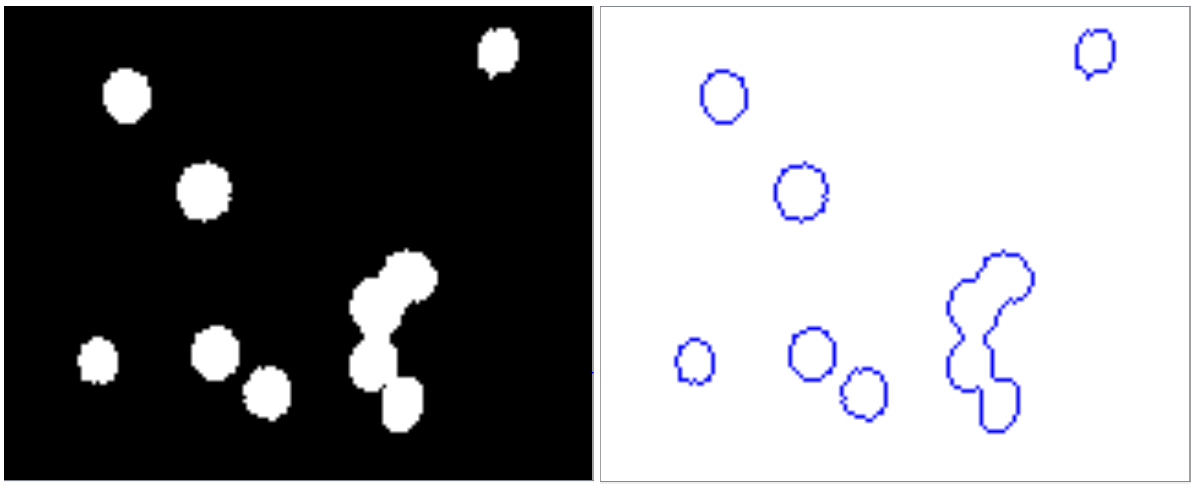
\includegraphics[width=150mm]{images/seg_bin_con.png}
\end{center}
\caption{Бинарна/црно-бела слика (лево) и означене контуре са слике (десно)}
\label{fig:cv}
\end{figure}

Како контуре трагова могу бити спојене  потребно је да даље процесирамо такве контуре како бисмо их раздвојили на контуре појединачних трагова. Даље процесирање, односно сегментација трагова, не врши се над свим контурама, већ само над оним чије ка\-рак\-те\-рис\-ти\-ке указују на то да би могле бити изграђене од више спојених трагова. Користе се ка\-рак\-те\-рис\-ти\-ке попут величине контуре, конвексности контуре, броју одступања од конвексности, највећем одступању од конвексности. Уколико наведене карактеристике контуре нису дале јасну назнаку да се ради о контури једног трага, испитују се тачке које су потенцијални центри спојених трагова.

\begin{figure}[htb]
\begin{center}
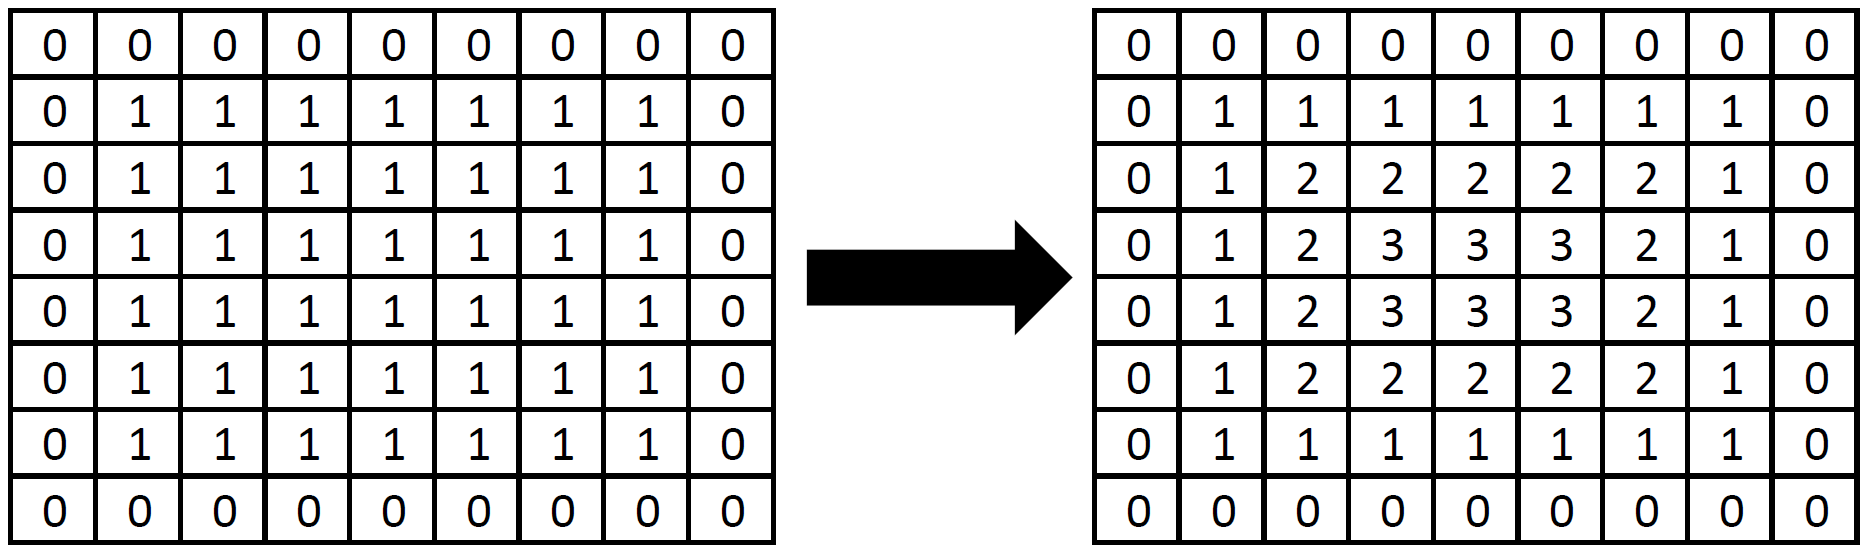
\includegraphics[width=120mm]{images/distance_matrix.png}
\end{center}
\caption{Матрица удаљености од позадине}
\label{fig:dist_matric}
\end{figure}

Потенцијалне центре спојених трагова тражимо на основу матрице удаљености од по\-за\-ди\-не. Матрица удаљености од позадине се обично рачуна само за бинарне слике, тако да  најпре извлачимо маску са бинарне слике трага који испитијемо, осносно најмањи квадрат са слике који садржи траг, а чије су ивице паралелне са ивицама слике. Над маском трага рачунамо матрицу удаљености (\textit{distance transform}). Резултат је сиво скалирана слика која личи на улазну слику, с тим да интензитети боја тачака унутар објеката показују удаљеност до најближе границе са позадином.

\begin{figure}[htb]
\begin{center}
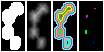
\includegraphics[width=150mm]{images/local_maxima.png}
\end{center}
\caption{(i) Бинарна маска трага; (ii) Матрица удаљености; (iii) Означене компоненте са матрице удаљености; (iv) Компоненте са матрице удаљености које представљају локалне максимуме вредности на матрици удаљености; }
\label{fig:local_maxima}
\end{figure}

Када израчунамо матрицу удањености, користимо \textit{connectedComponents} funkciju \textit{OpenCV}-ја да означимо засебне компоненте. Једна компонента представља све пикселе који се додирују, а притом имају исту вредност. Компоненте које представљају локалне максимуме користе се као потенцијални центри трагова.

 \begin{lstlisting}[language=C++,label=lst:local_maxima,caption=Проналажење централних региона трагова]
// Calculate distance matrix.
cv::Mat dist;
cv::distanceTransform(framedMask, dist, CV_DIST_L2, 5);

// Convers distance to integers.
cv::Mat dist_8u;
dist.convertTo(dist_8u, CV_8U);

// Mark local maximums and use it as hint for traces.
numberOfMarkers = MarkLocalMaximums(dist_8u, markers);
\end{lstlisting}

Уколико је детектован само један локални максимум, траг се ипак сматра засебним. У случају да је детектовано више локалних трагова, ради се сегментација, при чему се  локални максимуми користе као полазни региони за \textit{watershed} алгоритам.

\subsection{Сегментација трагова}

\textit{OpenCV} садржи модификовану верзију \textit{watershed} алгоритма. Имплементација не про\-на\-ла\-зи аутоматски регионе из којих креће да означава сличну околину, већ те регионе тражи као улазни параметар.Ту се користе локални максимуми одређени на основу матрице удањености. Добијене компоненте представљају детектоване трагове.

 \begin{lstlisting}[language=C++,label=lst:grayscaleOtsu,caption=Сегментација трагова]
// Markers are previously obtained local maximas.
// Mark background.
for (int r = 0; r < mask.rows; r++)
{
    for (int c = 0; c < mask.cols; c++)
    {
        int index = (int) mask.at<char>(r,c);
        if (index == 0)
        {
            markers.at<int>(r,c) = 255;
        }
    }
}

// Run watershed alghoritm to segment connected traces.
Mat result;
cvtColor(mask, result, CV_GRAY2BGR);
cv::watershed(result, markers);
\end{lstlisting}

\begin{figure}[htb]
\begin{center}
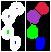
\includegraphics[width=75mm]{images/watershed.png}
\end{center}
\caption{Полазна и крајња матрица за \textit{watershed} алгоритам}
\label{fig:result}
\end{figure}

\section{Исправљање ротације слике у односу на претходну слику из секвенце}

При прикупљању секвенце слика у различитим временским тренуцима дешава се да материјал детектора није усликан под истим углом. У том случају, позиција истих трагова на различитим сликама није иста и није могуће пратити раст трагова. Зато приступамо отклаљаљу ротације (\textit{deskew}) слике у односу на предходну слику из секвенце.

\begin{figure}
\begin{center}
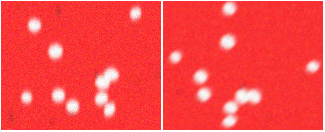
\includegraphics[width=150mm]{images/prev+new.png}
\end{center}
\caption{Претходна слика из секвенце (лево) и нова слика (десно)}
\label{fig:otsu}
\end{figure}

Пошто је могуће да ce трагови не шире у истом правцу и на исти начин, може да се деси и да се контуре трагова значајно разликују. Проналажење сличности између две сличне слике је део многих апликација рачунарског вида: калибрација камере, 3Д реконструкција, препознавање објеката и тако даље. Ови алгоритми се  углавном састоје од три главна корака:
\begin{enumerate}
  \item детекција интересних тачака,
  \item рачунање описног вектора у интересним тачкама и
  \item поређење описних вектора и одређивање трасформације.
\end{enumerate}

\subsection{Детекција интересних тачака}
Интересне тачке су препознатљиве тачке објекта које се могу пронаћи при различитим погледима на објекат. Описивањем ових тачака на такав начин да су независне од величине слике, ротације и осветљења, постиже се циљ уочавања сличности између различитих слика. Поређењем описних вектора може се донети закључак о трансформацији слике. Oвe тачке  се бирају на карактеристичним местима, као што су оштре ивице, мрље, Т-спојеви. 
У посматраном случају, алгоритам се ослања на чињеницу да се исти узорак слика у различитим временским тренуцима. Другим речима, на сликама ће бити присутни исти трагови и однос између суседних трагова ће остати исти. Због тога се за интересне тачке бирају центри детектованих трагова.

\subsection{Рачунање описног вектора}

Описни вектор представља вектор који описује околину интересне тачке. Овај вектор мора бити карактеристичан, отпоран на шум и дефекте који настају при фотографисању. Како се алгоритам ослања на претпоставку да у новој слици из секвенце нема превише нових трагова и новонасталог шума, описни вектор за сваку тачку се гради од сортираних удаљености центра дате тачке од центара пет најближих трагова.

\begin{figure}
\begin{center}
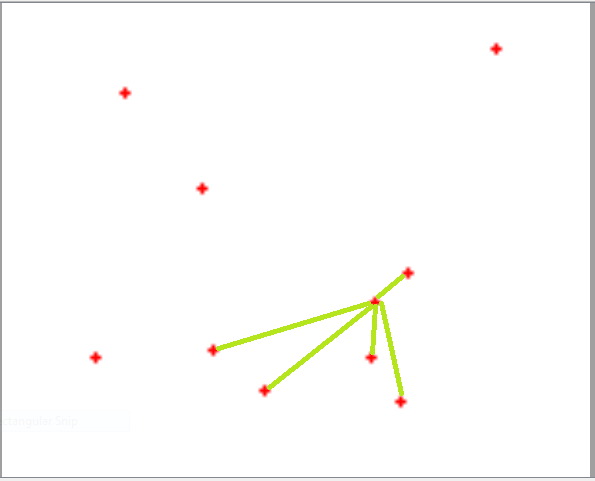
\includegraphics[width=100mm]{images/desc.png}
\end{center}
\caption{Вредности описног вектора једног трага}
\label{fig:desc}
\end{figure}

\subsection{Поређење описних вектора и одређивање трансформације}

На крају се врши упоређивање описних вектора, односно рачуна се еуклидско растојање између описног вектора интересне тачке са описним векторима свих интересних тачака друге слике.  Када се добије списак парова са најмањим растојањем, бира се најмање три, а највише десет тачака на основу којих се тражи матрица хомографије. \textbf{Хомографија} је пројекцијска трансформација којом се описују пресликавања тачке из једне равни у другу:
\begin{equation}
x \prime = H x,
\end{equation}
где су $x\prime$ и $x$ тачке у различитим равнима, а $H$ матрица трансформације која описује транслацију, ротацију, скалирање и перспективу. У датом случају, очекује се афина хо\-мо\-гра\-фи\-ја, односно да нема перспективе.

\begin{figure}[h]
\begin{center}
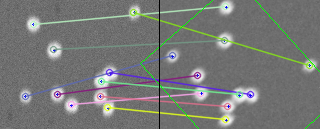
\includegraphics[width=150mm]{images/rotation.png}
\end{center}
\caption{Препознате тачке са најмањим еуклидским растојањем описних вектора и детектована трансформација}
\label{fig:rotation}
\end{figure}

\begin{lstlisting}[language=C++,label=lst:surf,caption=Поређење описних вектора и одређивање ротације нове слике]
Mat Document::CalcTransform(Document* prev, Document* curr)
{
    // Get traces for previous and current image.
    vector<Trace>& prevTraces = prev->GetTraces();
    vector<Trace>& currTraces = curr->GetTraces();

    // Get distance from 5 closest traces for both, previous and current image.
    Mat prevN5 = GetDist(prevTraces);
    Mat currN5 = GetDist(currTraces);

    // Match desctiption vectors.
    BFMatcher matcher;
    std::vector<DMatch> matches;
    matcher.match( prevN5, currN5, matches );

    // Pack matches in vector and sort them by distance,
    std::vector<DMatch*> refMatches = SortMatches(matches);

    // Get matching points witth least distance.
    std::vector<Point2f> pPrev;
    std::vector<Point2f> pCurr;
    for(size_t i = 0; i < matches.size() && i < 10; i++)
    {
        DMatch* m = refMatches[i];

        pPrev.push_back(getTraceCenter(prevTraces[m->queryIdx]));
        pCurr.push_back(getTraceCenter(currTraces[m->trainIdx]));
    }

    Mat transform;
    // Minimum 3 points to detect transformation.
    if (pCurr.size() >= 3 && pPrev.size() >= 3)
    {
        Mat temp = findHomography(pCurr, pPrev, CV_RANSAC);

        // Check is it affine homography.
        // h_{31}=h_{32}=0, \; h_{33}=1.
        double h31 = temp.at<double>(2,0);
        double h32 = temp.at<double>(2,1);
        double h33 = temp.at<double>(2,2);
        if (abs(h31) < cAlmostZero && abs(h32) < cAlmostZero && abs(h33 - 1) < cAlmostZero)
        {
            transform = temp;
        }
    }

    return transform;
}
\end{lstlisting}

Дати алгоритам функционише готово без грешке ако се примени на вештачки ге\-не\-ри\-са\-ним примерима. Међутим, у случају да су трагови превише густи, односно детекција не разреши спојене трагове, или у случају да на слици има веома мало трагова, може се очекивати да трансформација не буде успешно детектована. Алгоритам се може побољшати увођењем нових вредности у описни вектор интересних тачака, на пример: однос дужег и краћег дијаметра, углови који се формирају са најближим тачкама, а чије је теме у посматраној тачки итд. 

%%%%%%%%%%%%%%%%%%%%%%%%%%%%%%%%
%
% Поглавље 3:
%
% Развој корисничког интерфејса употребом Qt оквира
%
%%%%%%%%%%%%%%%%%%%%%%%%%%%%%%%%

\chapter{Развој корисничког интерфејса употребом \textit{Qt} оквира}

\textit{Qt} \cite{qt} је оквир за развој корисничког интерфејса. Омогућује развој апликација и за десктоп рачунаре и за мобилне телефоне, без потребе да се поново пише изворни код. \textit{Qt} је надскуп стандардног \textit{C++} програмског језика, тако да програмери могу да користе или \textit{Qt} или стандардне \textit{C++} библиотеке, а могу да се користе и у комбинацији.

\begin{figure}[htb]
\begin{center}
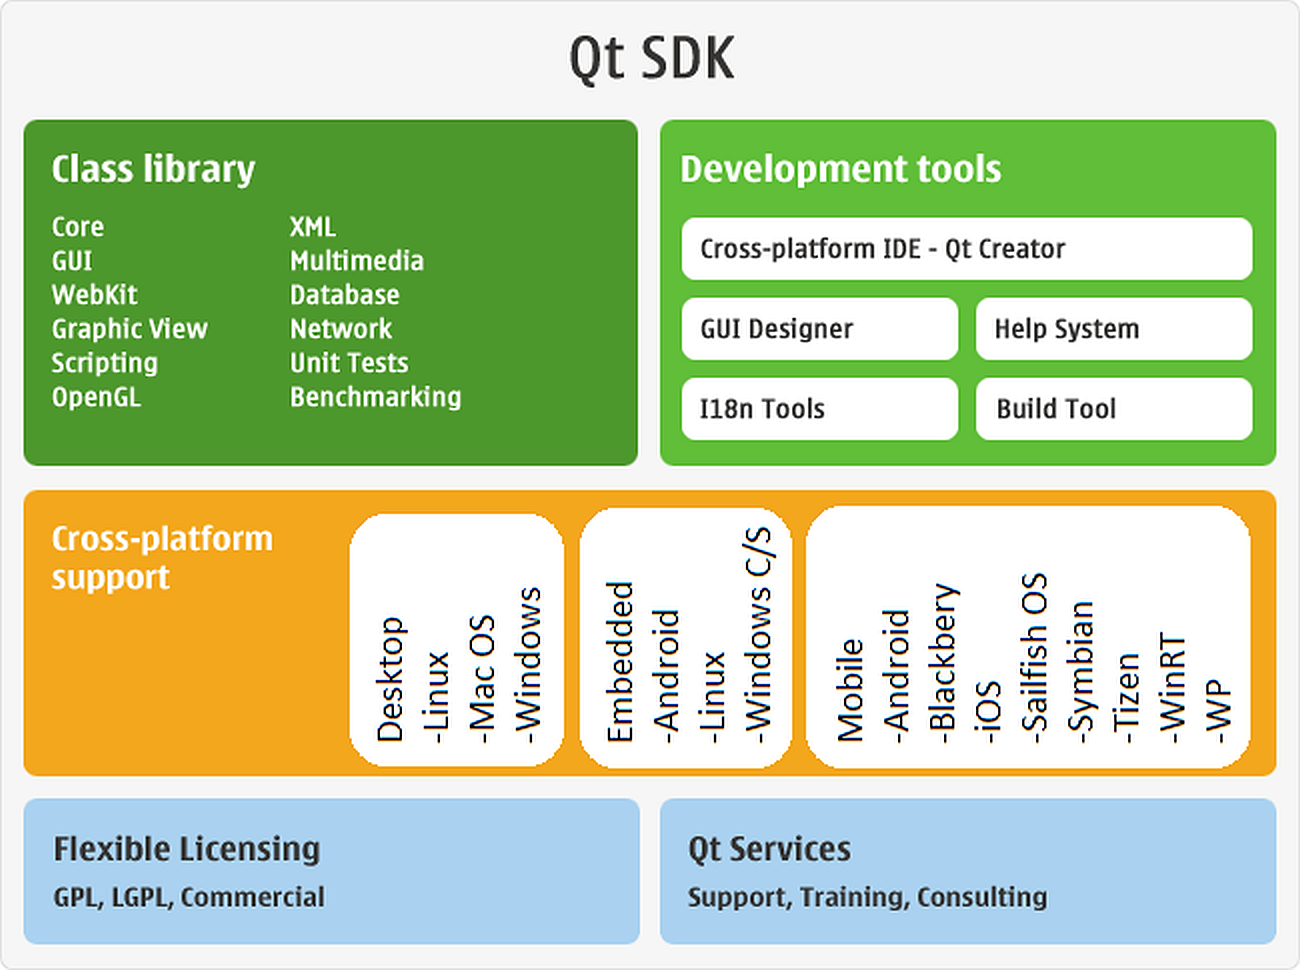
\includegraphics[width=150mm]{images/qt_platforms.png}
\end{center}
\caption{\textit{Qt SDK (Software Development Kit)}}
\label{fig:qtsdk}
\end{figure}

\textit{Qt} већ користе стотине хиљада програмера. Значајани делови \textit{Linux KDE} графичког окружења, \textit{Google Earth} и \textit{Skype} програма су написани коришћењем овог оквира. Обухвата богат скуп графичких контрола \textit{Widgets} које пружају стандарднe \textit{GUI} функционалности као што су менији, контекстни мени, \textit{drag and drop}, и слично. Уводи иновативну и безбеднију алтернативу за комуникацију између објеката названу \textit{Signals and Slots}, али подржава и конвенционални модел за реаговање на клик миша, притисак дугмета, и друге улазне догађаје.

Од самог почетка \textit{Qt} је био доступан за слободну комерцијалну употребу. То је омо\-гу\-ћи\-ло развој апликација без икаквих ограничења лиценцирања. Постојало је више различитих лиценци. У почетку изворни код је био под лиценцом \textit{FreeQT} која је дозвољавала пре\-у\-зи\-ма\-ње и употребу кода, али је објављивање модификација било забрањено. Тренутно, код је доступан под \textit{GNU Lesser General Public 2.1 (LGPL)}, која га чини доступним за употребу у пројектима и отвореног и затвоеног кода.

\section{Развојни алати}

\textit{Qt} нуди широк скуп алата за развој софтвера:
\begin{itemize}
  \item \textbf{\textit{Qt Assistant}} је алат који графички презентује \textit{HTML} документацију пројекта. Са\-држи примере кода и пуно корисних информација о томе како се користите класе оквира. Такође, пружа могућност једноставне претраге документације.

  \item \textbf{\textit{Qt Designer}} је алат за пројектовање и изградњу корисничког интерфејса. Ко\-ри\-сни\-чки интерфејс се развија на \textit{what you see what you get (WYSWYG)} начин. Могуће је тестирање понашања интерфејса при различитим резолуцијама, што олакшава развој на различитим платформама. Визуелне контроле креиране са овим дизајнером интегришу се са програмским кодом употребом модела сигнала и слотова што олакшава раздвајање функционалности од корисничког интерфејса. Све карактеристике ви\-зу\-ел\-них контрола се могу мењати и динамички у коду. Информације о корисничком интерфејсу се чувају у фајловима са екстензијом \textit{.ui}. То су \textit{XML} фајлови на основу којих се аутоматски генерише \textit{C++} код који се даље компајлира.

  \item \textbf{\textit{Qt Linguist}} је алат који омућава локализацију апликације.

  \item \textbf{\textit{Qt Creator}} је развојно окружење \textit{(IDE - Integrated Development Environment)} које интегрише претходно наведене алате. Такође, пружа алате за извршавање задатака током целог циклуса развоја апликације. Аутоматизује и убрзава задатке као што су креирање пројеката, додавање нових фајлова, нуди семантичко означавање, проверу синтаксе кода, комплетирање наредбе, рефакторисање, као и многе друге корисне функције.
\end{itemize}

\section{Модули}

\textit{Qt} фрејмворк је подељен у неколико засебних модула. Да би се користиле фун\-кци\-о\-нал\-но\-сти одређеног модула, потребно је додати одговарајућу променљиву у пројектни фајл. На пример, за употребу класа за рад са \textit{XML} фајловима потребно је додати:
\begin{lstlisting}[language=C++,label=lst:pro,caption=Укључивање модула за рад са \textit{XML} фајловима]
QT += xml;
\end{lstlisting}

Коришћени модули за приказ корисничког интерфејса у софтверу за детекцију трагова неутронске дозиметрије обухватају:
\begin{itemize}

  \item \textbf{\texttt{QtCore}} садржи основне класе које користи свака \textit{Qt} апликација, као и други модули. Овај модул омогућава рад са објектима (\texttt{QObject)}, стринговима (\texttt{QString)}, фајловима (\texttt{QFile)}, фолдерима (\texttt{QDir}), локализацијом (\texttt{QLocаle)} и тако даље. Овај модул је подразумеван, тако да га није потребно експлицитно укључивати.

  \item \textbf{\texttt{QtGui}} модул садржи компоненте графичког корисничког интерфејса (\textit{GUI}). Садржи специјализоване контроле \texttt{Widgets} (\texttt{QCalendarWidget}, \texttt{QDockWidget}), кон\-теј\-не\-ре \\ (\texttt{QGroupBox}, \texttt{QStackedWidget}) и дијалоге (\texttt{QFileDialog}, \texttt{QPrintDialog}).

  \item \textbf{\texttt{QtXml}} садржи класе за рад са \texttt{Xml} фајловима. Омогућава читање, писање и фор\-ма\-ти\-ра\-ње \texttt{Xml} структура.

\end{itemize}

\section{Сигнали и слотови}

Сигнали и слотови (\textit{Signals and Slots}) су основни механизам свих \textit{Qt} програма. Омо\-гу\-ћа\-ва\-ју комуникацију између објеката који не знају ништа једни о другима. Типичан пример је када желимо да промена у једној од контрола утиче на промене у другој контроли. Само наслеђене класе из \textit{QtObject} могу применити механизам сигнала и слотова. \textit{Widget} контроле имају пуно предефинисаних сигнала и слотова, али је могуће додефинисати нове по потреби.

Идеја је да један објекат може да пошаље сигнал са информацијама насталој промени без знања да ли ће ту информацију неко прихватити. Други објекти се могу повезати на ту врсту сигнала, и при емитовању сигнала од стране првог објекта могу извести одређену акцију. Могуће је повезати само сигнале и слотове са истим параметрима. Слотови се коористе за пријем сигнала. У суштини, то су обичне \textit{C++} функције, тако да се могу извршити у било које време.

\begin{lstlisting}[language=C++,label=lst:signal_and_slot,caption=Дефиниција и емитовање сигнала]
class Sender : public QObject
{
    Q_OBJECT

public:
    void sendSignal()
    {
         // Emit signal.
         emit newMessage("Message text!");
    }

signals:
    void newMessage(QString message);
};
\end{lstlisting}

\begin{lstlisting}[language=C++,label=lst:signal_and_slot,caption=Дефиниција слота]
class Receiver : public QObject
{
    Q_OBJECT

public slots:
   receiveMessage(QString message)
    {
        // Print received message to debug console.
        qDebug() << message;
    }
};
\end{lstlisting}

Сигнали и слотови се могу повезати на следећи начин:

\begin{lstlisting}[language=C++,label=lst:signal_and_slot,caption=Повезивање сигнала и слотова]
QObject::connect(
    sender,
    SIGNAL(newMessage),
    receiver,
    SLOT(receiveMessage));
\end{lstlisting}

На један сигнал могуће је прикачити више слотова. Чекање на сигнал се може и укинути:

\begin{lstlisting}[language=C++,label=lst:signal_and_slot,caption=Укидање везе сигнала и слота]
QObject::disconnect(
    sender,
    SIGNAL(newMessage),
    receiver,
    SLOT(receiveMessage));
\end{lstlisting}

%%%%%%%%%%%%%%%%%%%%%%%%%%%%%%%%
%
% Поглавље 4:
%
% Софтвер за детекцију трагова неутронске дозиметрије
%
%%%%%%%%%%%%%%%%%%%%%%%%%%%%%%%%

\chapter{Софтвер за детекцију трагова}

\textit{Софтвер за детекцију трагова неутронске дозиметрије} омогућава обраду слика не\-у\-трон\-ске дозиметрије добијених употребом детектора \textit{CR-39}. Резултат употребе софтвера је добијање информација о броју трагова неутрона, њиховој позицији и величини. Омогућено је подешавање параметара обраде слика, подешавање приказа, као и чување резултата обраде. Софтвер је намењен истраживачима са Института за физику Природно-мате\-ма\-ти\-чког факултета Универзитета у Крагујевцу, који се баве проценом дозе апсорбованог неутронског зрачења.

Обрада слике je веома сложенa и захтевна по питању перформанси. Услед предности у брзини у односу на неке друге платформе, софтвер је комплетно развијен у програмском језику \textit{C++}. Поред стандардних библиотека \textit{C++} језика, коришћена је \textit{OpenCV} библиотека за обраду слика, као и \textit{QT} платформа за развој корисничког интерфејса. Као такав, софтвер је портабилан, а тестиран је на \textit{Ubuntu 14.04 LTS} и \textit{Windows 7/8.1/10} оперативним системима.

\begin{figure}[H]
\begin{center}
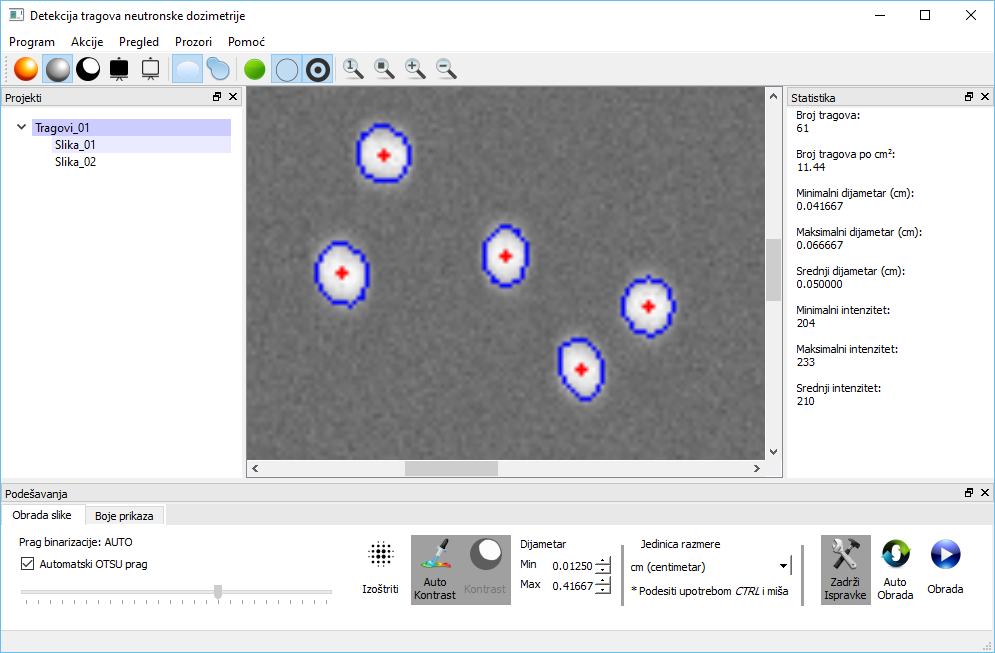
\includegraphics[width=135mm]{images/softver.png}
\end{center}
\caption{Софтвер за детекцију трагова неутронске дозиметрије}
\label{fig:softver}
\end{figure}

\section{Структура пројекта}
Изворни код софтвера налази се на адреси \texttt{https://github.com/nik0la31/Application-of-pattern-recognition-algorithms-in-neutron-dosimetry}. Изворни код је подељен у две целине, односно два пројекта: \texttt{ndtr\_engine} и \texttt{ndtr\_app}, које су задужене за детекцију трагова неутронске до\-зи\-ме\-три\-је обрадом слике и графички кориснички интерфејс, респективно.

\begin{figure}[H]
\begin{center}
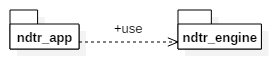
\includegraphics[width=60mm]{images/struktura.png}
\end{center}
\caption{Структура пројекта}
\label{fig:struktura}
\end{figure}

Пројекат \textit{ndtr\_app} садржи свега четири класе:

\begin{itemize}
  \item \texttt{MainWindow} класа садржи дизајн корисничког интерфејса и управља интеракцијом са корисником;
  \item \texttt{Workspace} класа представља модел у \textit{Model/View} архитектури. Чува све релевантне податке о учитаним пројектима и сликама, тренутном приказу, одабраним по\-де\-ша\-ва\-њи\-ма и слично;
  \item \texttt{ProjectItem} је изведен из \textit{QT} класе \texttt{QStandardItem} и дефинише специфично по\-на\-ша\-ње чворова пројеката и докумената (слика) у хијерархијском приказу;
  \item \texttt{ProjectParser} је класа задужена за чување и учитавање пројеката.
\end{itemize}

Пројекат \texttt{ndtr\_engine} представља срж апликације и садржи следеће типове:

\begin{itemize}
  \item \texttt{Contour} описује контуру трага, односно садржи вектор тачака који описује траг.
  \item \texttt{Ellipse} описује најмању елипсу која се може описати око детектованог трага. Де\-фи\-ни\-са\-на је центром, два дијаметра, и углом.
  \item \texttt{ShapeType} енумерација дефинише који се облици трага могу приказати (контура, елипса).
  \item \texttt{ImageType} енумерација дефинише који се типови слике могу приказати (изворна, сиво скалирана, црно бела, са црном позадином, са белом позадином).
  \item \texttt{ViewOptions} структура се користи да се задају опције приказа да би се генерисала одговарајућа слика. 
  \item \texttt{ProcessingOptions} структура служи за задавање подешаваља обраде слике. Могућа подешавања су: употреба аутоматског \textit{Otsu} прага бинаризације, задавање конкретног прага бинаризације, изоштравање слике, дефинисање односа контраста трагова у односу на позадину, односно бели трагови на тамној позадини или супротно (\textit{WoB - white on black}).
  \item \texttt{Trace} структура описује детектовани траг. Траг је дефинисан са два дијаметра, углом, \textit{x} и \textit{y} координатама центра трага, просечним интензитетом боје.
  \item \texttt{Stats} структура садржи статистичке податке који се рачунају за сваку слику: Нај\-ма\-њи, највећи и просечни дијаметар трага, најмањи, највећи и просечни интензитет боје трага.
  \item \texttt{Document} класа садржи методе за детекцију трагова. Такође, садржи методу за детекцију трансформације, односно угла између две слике у секвенци. Ослања се на \textit{OpenCV} библиотеку.
  \item \texttt{Project} класа садржи документе, оснодно слике са процесуираним подацима. Води рачуна о додавању, брисању и  редоследу докумената у пројекту.
\end{itemize}

\begin{figure}[H]
\begin{center}
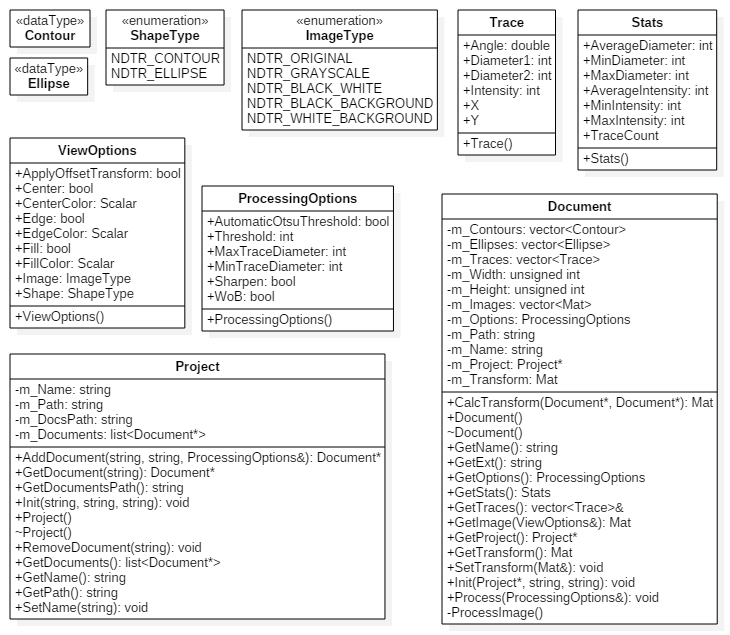
\includegraphics[width=150mm]{images/engine.png}
\end{center}
\caption{Дијаграм класа \textit{ndtr\_engine} пројекта}
\label{fig:engine}
\end{figure}

\section{Начин употребе}

Кориснички интерфејс је једноставан за коришћење и прегледан, тако да је корисницима омогућено брзо прилагођавање на рад овим алатом. На слици \ref{fig:softver2} је приказан кориснички интерфејс програма. Подељен у пет главних целина:
\begin{enumerate}
  \item Приказ и визуелизација детектованих трагова.
  \item Опције приказа детектованих трагова.
  \item Управљање пројектима и сликама.
  \item Опције обраде слике.
  \item Приказ података добијених обрадом слике.
\end{enumerate}

\begin{figure}[H]
\begin{center}
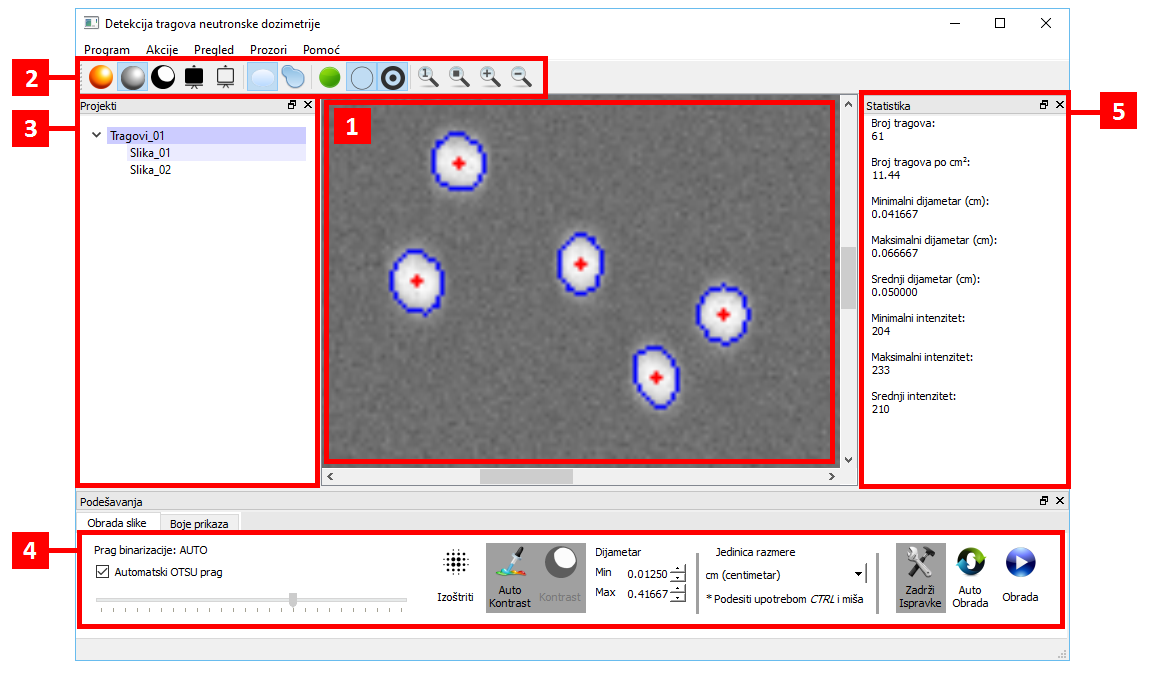
\includegraphics[width=150mm]{images/softver2.png}
\end{center}
\caption{Основне компоненте софтвера за детекцију трагова неутронске дозиметрије}
\label{fig:softver2}
\end{figure}

\subsection{Управљање пројектима}

Контрола за управљање пројектима омогућава креирање, отварање, затварање и чување пројеката.
Пројекат служи као контејнер који групише слике неутронске дозиметрије у јединствену целину.
Такође, кроз ову контролу врши се и додавање и брисање слика неутронске дозиметрије из пројекта. Структура пројекта на диску је следећа:

\begin{tabbing}
NazivProjekta.ndtr \\
<Naziv\= Projekta>   \\
\>    NazivSlike.ext \\
\>    . . . \\
\end{tabbing}

У директоријуму који носи назив пројекта налазе се све слике се које користе у пројекту, а истоимена датотека са екстензијом \textit{.ndtr} садржи и дефиницију пројекта.

\begin{lstlisting}[language=Xml,label=lst:Project,caption=Пример дефиниције пројекта]
<?xml version="1.0" encoding="UTF-8"?>
<ndtr>
    <documents>
        <document name="Slika_01" ext=".png">
            <options AutomaticOtsuThreshold="1" OtsuThreshold="160" Sharpen="0" WoB="1" MinTraceDiameter="5" MaxTraceDiameter="40"/>
        </document>
        <document name="Slika_02" ext=".png">
            <options AutomaticOtsuThreshold="1" OtsuThreshold="161" Sharpen="0" WoB="1" MinTraceDiameter="5" MaxTraceDiameter="40"/>
        </document>
    </documents>
</ndtr>
\end{lstlisting}

\begin{figure}[H]
\begin{center}
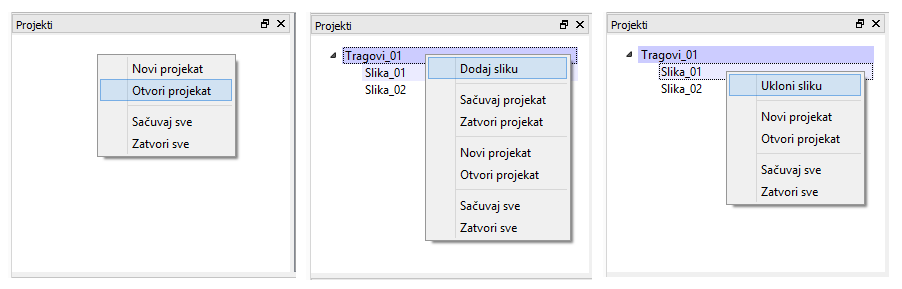
\includegraphics[width=150mm]{images/projects.png}
\end{center}
\caption{Контрола за управљање пројектима и опције менија}
\label{fig:projects}
\end{figure}

\subsection{Приказ и опције приказа детектованих трагова}

У централном делу корисничког интерфејса налази се приказ слике неутронске дозиметрије и де\-тек\-то\-ва\-них трагова. Изнад се налазе опције приказа којима се управља шта се заправо приказује и шта је означено на приказу.

\begin{figure}[H]
\begin{center}

\includegraphics[width=150mm]{images/viewoptions.png}
\end{center}
\caption{Опције приказа}
\label{fig:viewoptions}
\end{figure}

Први сет опција дефинише тип слике која се приказује. Могуће је одабрати изворну слику, сиво скалирану слику, црно-белу слику, слику са црном позадином и слику са белом позадином. Приказ различитих типова слика може бити користан да упути на могућу корекцију параметара за обраду слика.

\begin{figure}[H]
\begin{center}
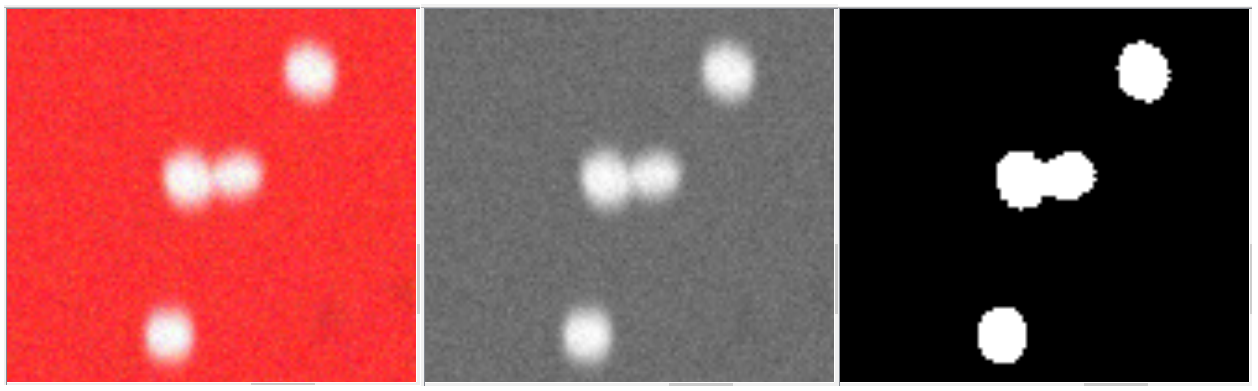
\includegraphics[width=150mm]{images/imagetype.png}
\end{center}
\caption{Опције приказа: изворна, сиво скалирана и црно-бела слика}
\label{fig:imagetype}
\end{figure}

Други сет опција дефинише у ком облику треба приказати детектовани траг. Могуће опције су контура или елипса.

\begin{figure}[H]
\begin{center}
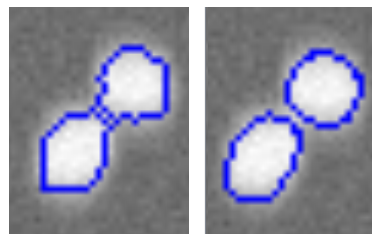
\includegraphics[width=80mm]{images/shapetype.png}
\end{center}
\caption{Опције приказа: контура трага или елипса која описује траг}
\label{fig:shapetype}
\end{figure}

Наредни сет опција дефинише како се детектовани траг означава на приказу. Могуће је означити ивицу, целу површину, као и центар трага. У контроли за подешавања, могуће је одредити којим се бојама приказују трагови на слици.

\begin{figure}[H]
\begin{center}
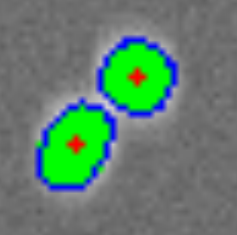
\includegraphics[width=40mm]{images/trace.png}
\end{center}
\caption{Опције приказа: ивица је приказана плавом, површина зеленом, а центар трага црвеном бојом}
\label{fig:trace}
\end{figure}

\begin{figure}[H]
\begin{center}
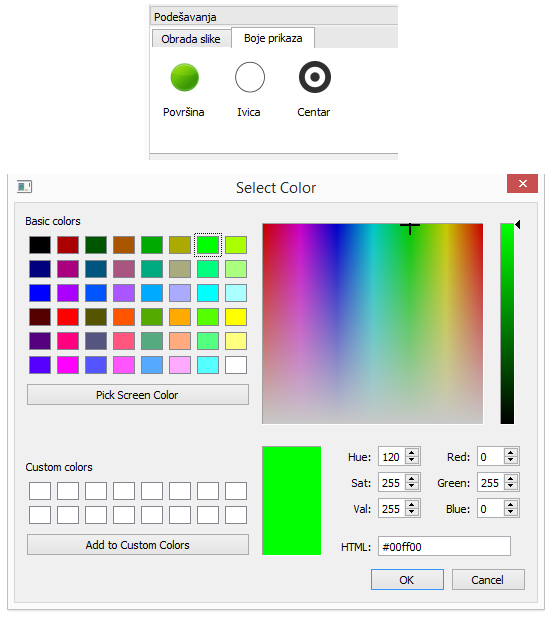
\includegraphics[width=130mm]{images/colors.png}
\end{center}
\caption{Подешавања: одабир боја приказа трагова}
\label{fig:colors}
\end{figure}

Последњи сет опција тиче се величине приказане слике. Слику је могуће увећати, умањити, приказати у изворној величини или је приказати целу на доступној површини контроле.

Тренутни приказ се може копирати или сачувати одабиром одговарајућих наредби из менија \texttt{Акције -> Копирај слику}, односно \texttt{Акције -> Сачувај слику}.

\subsection{Приказ и извоз резултата обраде}

Контрола за преглед резултата обраде слике пружа основне податке о детектованим траговима. Приказани су подаци попут укупног броја трагова, величине најмањег, највећег и средњег дијаметра трага као и најмањег, највећег и средњег интензитета боје трага. 

\begin{figure}[H]
\begin{center}
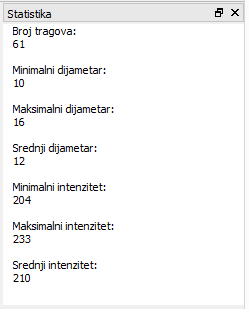
\includegraphics[width=60mm]{images/stats.png}
\end{center}
\caption{Контрола за приказ резултатa обраде слике}
\label{fig:stats}
\end{figure}

Кликом на одрећени траг из приказа, добијају се и основне инфомације датог трага попут позиције, величине и интензитета боје. Подаци везани за целу слику и за сваки детектовани траг појединачно могу се сачувати у \textit{.csv} датотеку наредбом \texttt{Акције -> Извоз} из менија програма. 

\begin{lstlisting}[language=Xml,label=lst:stats,caption=Пример сачуваних резултата]
Broj tragova,
61,
Statistika,
Diajmetar,
Min,Max,Avg
10,16,12,
Intenzitet,
Min,Max,Avg
204,233,210,
Tragovi,
x,y,ugao,dijametar1,dijametar2,intenzitet,
260,463,172.956,12,14,211,
199,454,128.87,12,14,209,
. . .
\end{lstlisting}

\subsubsection{Подешавање параметара и обраде слике}

На посебној контроли налазе се доступна подешавања обраде слике и контроле којима се обрада покреће.
Доступна подешавања су: укључивање \textit{Otsu} прага бинаризације, задавање прага бинаризације, изоштравање слике, као и одређивање да ли су трагови светлији или тамнији у односу на позадину (\textit{Контраст} претпоставља детекцију светлих трагова на тамној позадини). Такође, детектоване трагове могуће је филтрирати према величини, односно могуће је задати најмањи и највећи дозвољени дијаметар трага. 

\begin{figure}[H]
\begin{center}
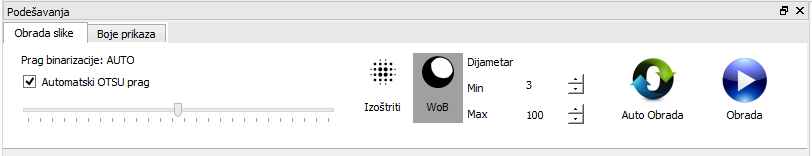
\includegraphics[width=150mm]{images/processing.png}
\end{center}
\caption{Контрола за подешавање и покретање обрада слике}
\label{fig:processing}
\end{figure}

Поред наведених подешавања, на контроли се налазе и команде за покретање об\-ра\-де, као и опција за аутоматску обраду при промени било ког параметра.

\subsubsection{Корекција детектованих трагова}

Како је могуће да програм погрешно класификује траг или шум. односно да не направи добру поделу између трагова, омогућена је мануелна исправка.

Уколико је траг погрешно класификован, десним кликом на траг приказује се мени из којег се могу одабрати опције \textit{Означи траг} или \textit{Означи шум}.

\begin{figure}[H]
\begin{center}
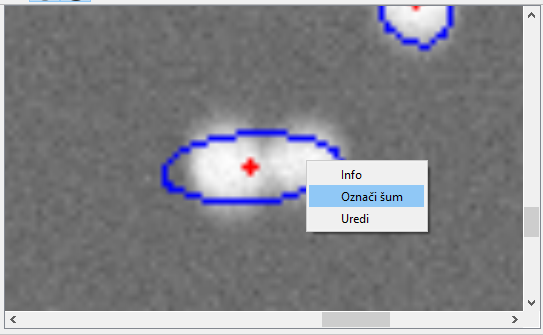
\includegraphics[width=100mm]{images/oznaci.png}
\end{center}
\caption{Корекција класификације траг-шум}
\label{fig:mark}
\end{figure}

Уколико граница између трагова није тачна, опција из менија \textit{Уреди} омогућава мануелно одређивање граница и класификовање трагова.

\begin{figure}[H]
\begin{center}
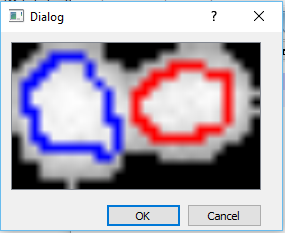
\includegraphics[width=75mm]{images/uredi.png}
\end{center}
\caption{Корекција трагова}
\label{fig:mark}
\end{figure}

Десним кликом се обележавају трагови (плава боја). Левим кликом се обележава шум (црвена боја). Није потребно означити цео траг, већ само приближне границе.
Означени делови се користе као полаз за претходно описани \textit{Watershed} алгоритам. У сличају погрешне ознаке, означени траг се може и обрисати средњим кликом.

%%%%%%%%%%%%%%%%%%%%%%%%%%%%%%%%
%
% Поглавље 5:
%
% Анализа
%
%%%%%%%%%%%%%%%%%%%%%%%%%%%%%%%%

\chapter{Анализа}

За мерење и вредновање детекције трагова неутронске дозиметрије генерисана су четири тест скупа по сто слика. Број трагова, њихова позиција и величина генерисани су насумице у задатом опсегу за сваку тест слику. Сваки тест скуп прављен је налик на репрезентативне примере пронађене на вебу, као и оне добијене од стране истраживача. Први тест скуп слика садржи светле трагове на тамној подлози. Други тест скуп садржи слике са тамним траговима који имају сенку у средњем делу. Трећи и четврти скуп садрже тамне трагове на светлијој позадини, с тим да је контраст интензитета боје између трагова и позадине већи у трећем скупу слика.

\begin{figure}[h]
\begin{center}
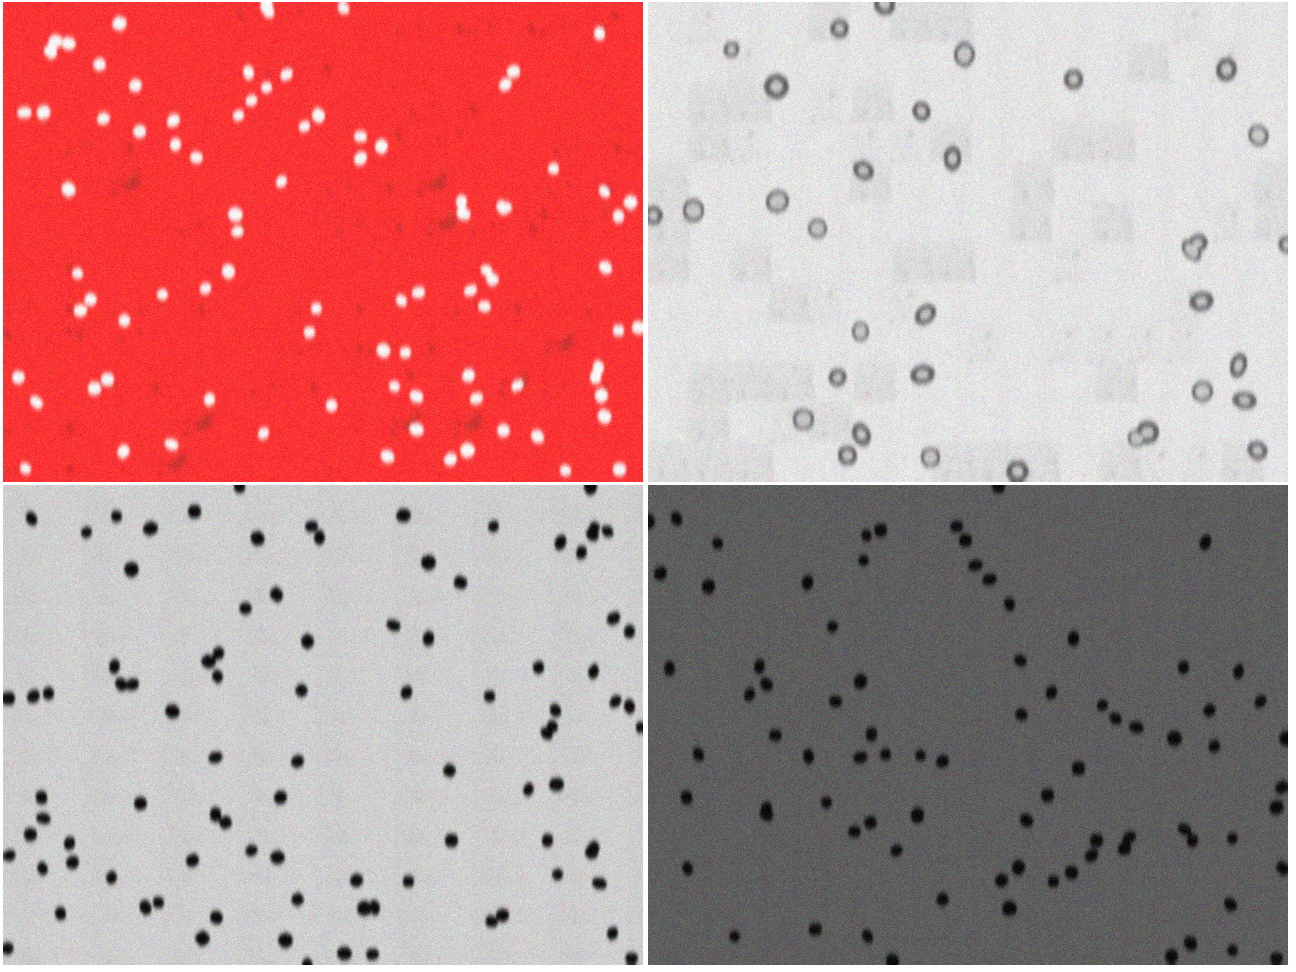
\includegraphics[width=150mm]{images/test.png}
\end{center}
\caption{Примери слика из тест скупова: (горе-лево) први тест скуп, (горе-десно) други тест скуп, (доле-лево) трећи тест скуп и (доле-десно) четврти тест скуп.}
\label{fig:test}
\end{figure}

\section{Резултати}

Као метрике за вредновање користе се \textit{тачност} и \textit{прецизност} система. \textit{Тачност} пред\-став\-ља однос исправно детектованих трагова према стварном броју трагова, док \textit{прецизност} представља однос исправно детектованих трагова према укуном броју детектованих трагова.

\begin{figure}[H]
\begin{center}
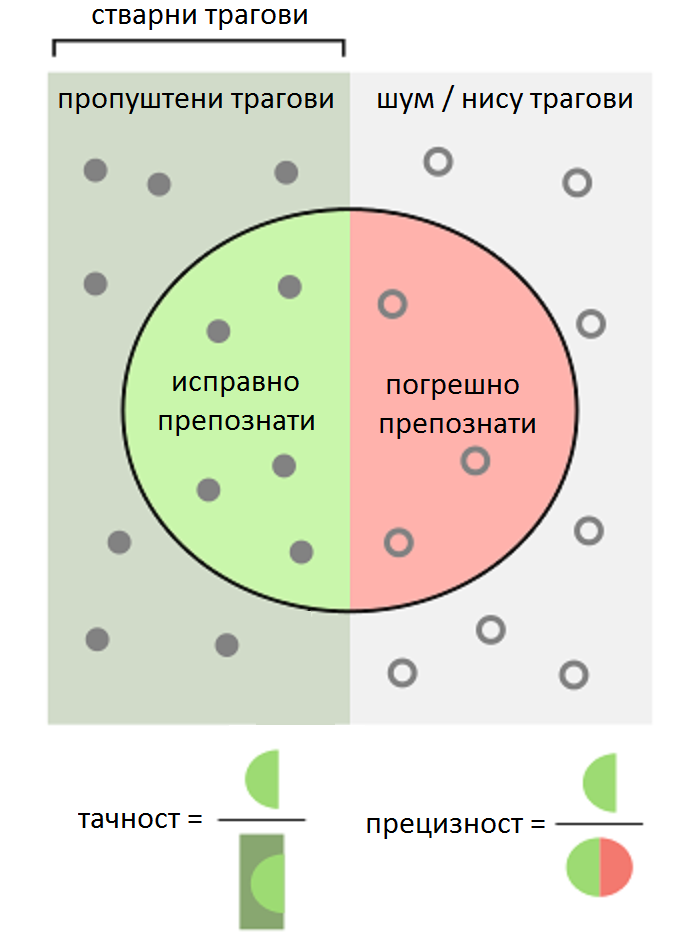
\includegraphics[width=120mm]{images/recall_prec.png}
\end{center}
\caption{Тачност и прецизност}
\label{fig:recall_prec}
\end{figure}

Написан је и програм који за сваку слику учитава податке о генерисаним траговима, извршава детекцију трагова и врши поређење. Резултат извршења програма су \textit{тачност} и \textit{прецизност} на новоу целог тест скупа, а такође и на нивоу сваке појединачне тест слике, уз генерисану слику са назначеним грешкама ради лакше анализе.

\begin{figure}[H]
\begin{center}
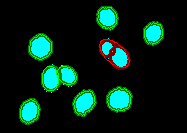
\includegraphics[width=100mm]{images/analysis.png}
\end{center}
\caption{Анализа слике: зелено означени трагови су препознати исправно, црвено означени трагови су препознати погрешно (cветло црвено означава шта је детектовано, а тамно црвено стварне трагове) }
\label{fig:analysis}
\end{figure}

При мерењу тачности и прецизности одабран је \textit{Otsu} аутоматски праг за бинаризацију, а остала подешавања попут изоштравања слике нису укључена.

\begin{table}[H]
\centering
\caption{Тачност и прецизност софтвера за детекцију неутронске дозиметрије}
\begin{tabular}{lrrrrrr}
\hline
& & & \multicolumn{2}{c}{Без сегментације} & \multicolumn{2}{c}{Са сегментацијом} \\
Тест скуп & Број слика & Број трагова & Тачност & Прецизност & Тачност &  Прецизност \\
\hline
Први & 100 & 6437 & 0.85 & 0.88 & 0.95 & 0.97 \\
Други & 100 & 4418 & 0.74 & 0.79 & 0.92 & 0.95 \\
Трећи & 100 & 6349 & 0.86 & 0.88 & 0.94 & 0.97 \\
Четврти & 100 & 6297 & 0.84 & 0.87 & 0.93 & 0.97 \\
\hline
\end{tabular}
\label{tab:metrics}
\end{table} 

\begin{figure}[H]
\begin{center}
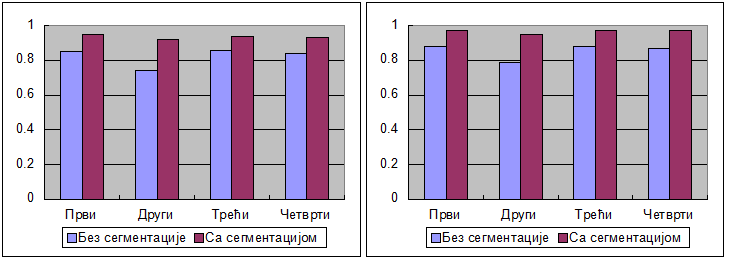
\includegraphics[width=150mm]{images/segmentation_results.png}
\end{center}
\caption{Утицај сегментације на тачност (лево) и прецизност (десно)}
\label{fig:seginf}
\end{figure}

\section{Најчешће грешке}

Најчешће грешке у детекцији трагова неутронске дозиметрије приказане су на сликама \ref{fig:error_overlapped}, \ref{fig:binthresh}, \ref{fig:multi}, \ref{fig:small} и \ref{fig:shadow}. Грешке углавном настају када се два или више  трагова превише преклапају. У једном делу таквих случајева промена прага бинаризације може помоћи. Међутим, код других трагова то може довести до тога да детектовани траг буде значајно мањи од реалног трага. Код дела преклопљених трагова на којима детектор греши, границе трагова нису видљиве ни за људско око. Код преклопљених трагова проблем је и процена величине трага, тј. део трага је сакривен иза једног или више других трагова и не изврши се задовољавајућа процена његове величине.

Додатно, код трагова са сенком у средишњем делу долази до тога да је траг, односно прстен трага сувише танак и да се сенка споји са позадином, чинећи да контура трага не буде затворена и за последицу препознта као више мањих трагова. Код преклапајућих трагова који имају сенку у средишњем делу није искоришћено само то својство да сенка може указати на центар трага. 


\begin{figure}[H]
\begin{center}
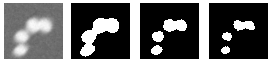
\includegraphics[width=150mm]{images/binthresh.png}
\end{center}
\caption{Код сегментације преклопљених трагова праг бинаризације битно утиче на исход. (i) Сиво скалирана слика. (ii) \textit{Otsu}  праг бинаризације (у датом случају 170) није увек одговарајући. (iii) У датом случају промена прага бинаризације на 190 даје боље резултате. (iv) Превише висок праг бинаризације (210) узрокује да детектовани трагови буду значајно мањи од реалних. }
\label{fig:binthresh}
\end{figure}

\begin{figure}[H]
\begin{center}
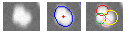
\includegraphics[width=150mm]{images/multi.png}
\end{center}
\caption{Грешка када се преклапа пуно трагова који формирају један велики траг. (i) Сиво скалирана слика. (ii) Детектовани траг.  (iii) Генерисани трагови. }
\label{fig:multi}
\end{figure}

\begin{figure}[H]
\begin{center}
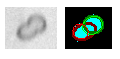
\includegraphics[width=150mm]{images/small.png}
\end{center}
\caption{Код преклопљених трагова тешко се одређује права величина трага. (i)  Сиво скалирана слика. (ii) Слика из анализе: Зелено означени траг је исправно препознат. Црвено означени траг се не рачуна као исправно детектован траг. Светло црвени је детектовани, а тамно црвени генерисани траг. }
\label{fig:small}
\end{figure}

\begin{figure}[H]
\begin{center}
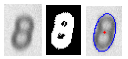
\includegraphics[width=150mm]{images/shadow.png}
\end{center}
\caption{Грешка при сегментацији преклопљених трагова где би податак о сенци у средини трага могао да помогне при детекцији. (i) Сиво скалирана слика. (ii) Бинарна слика. (iii) Детектовани траг. }
\label{fig:shadow}
\end{figure}

\begin{figure}[H]
\begin{center}
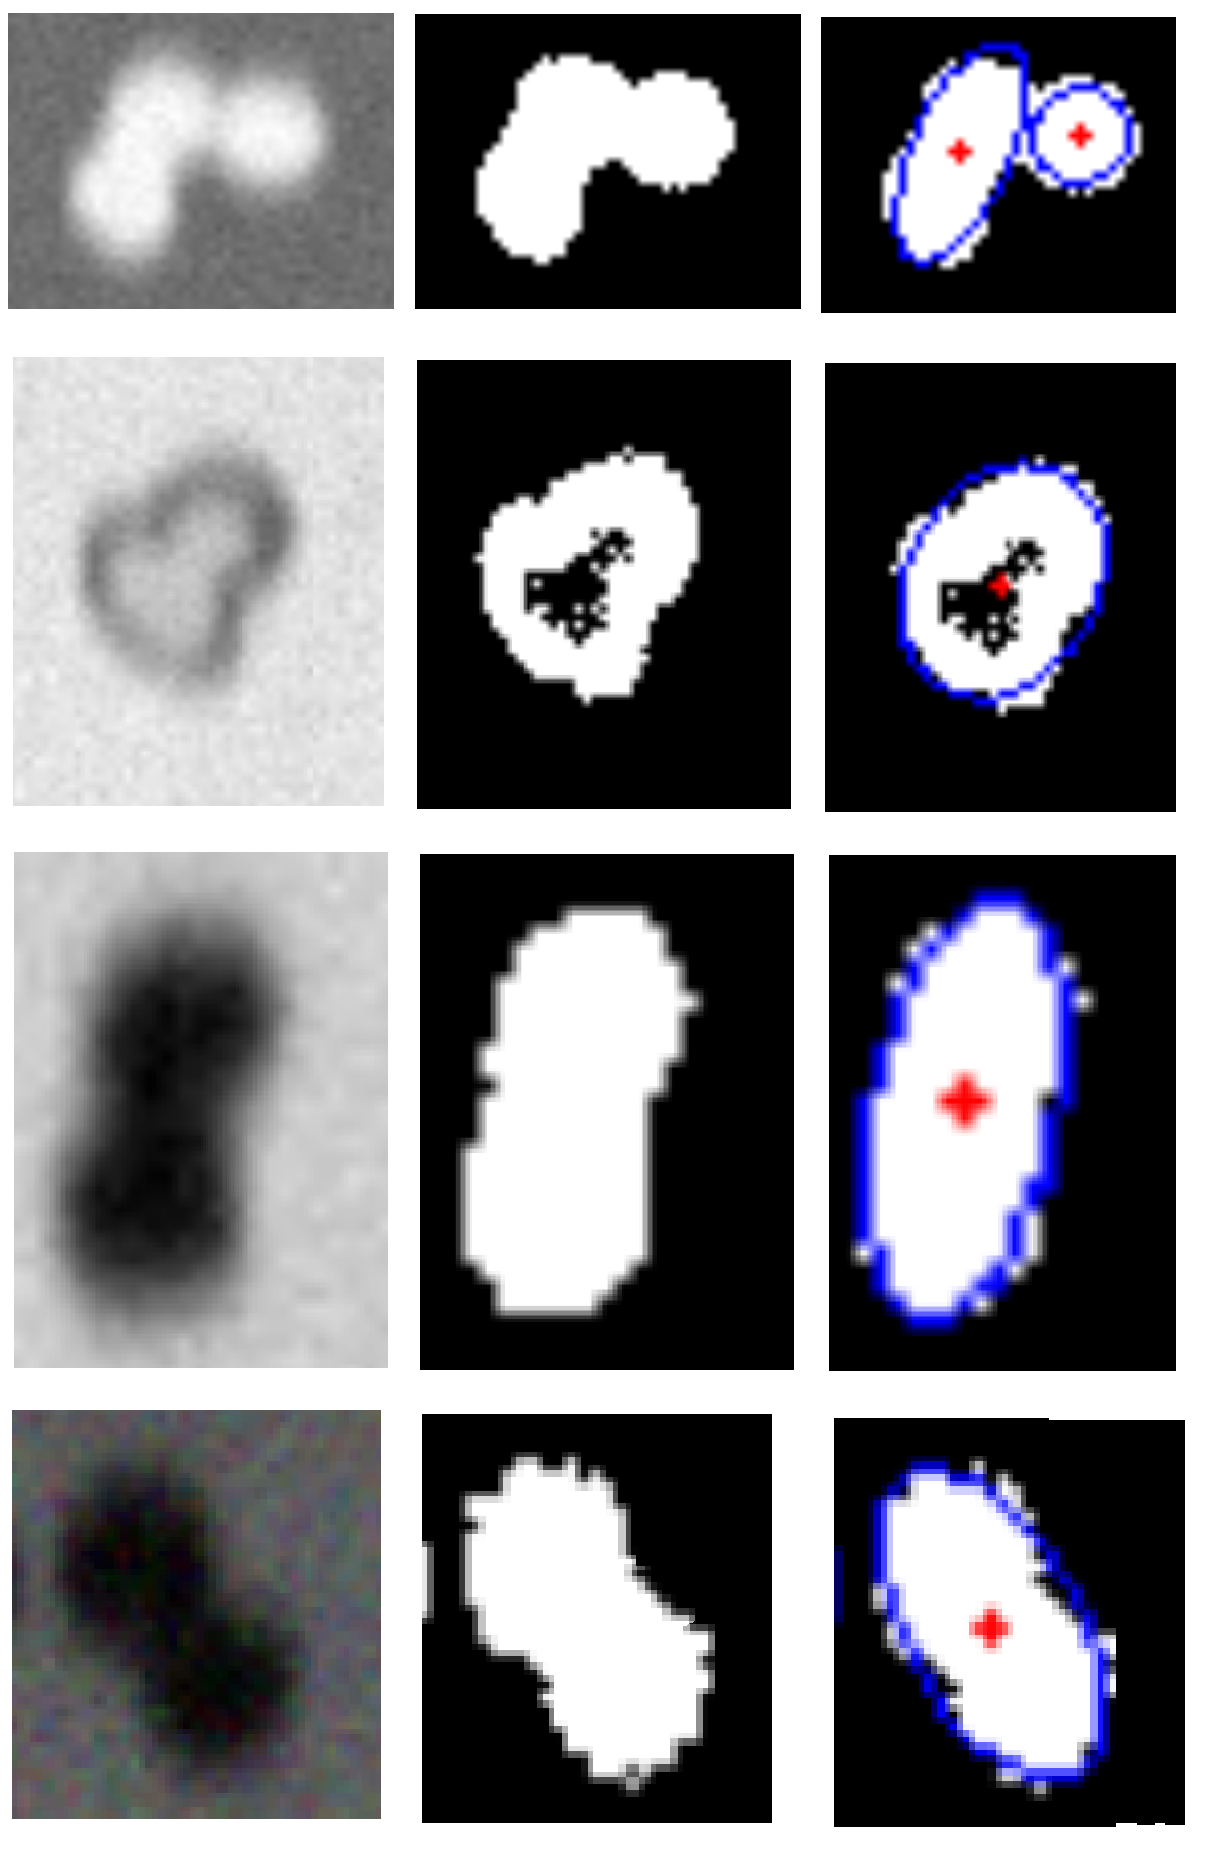
\includegraphics[width=150mm]{images/error01.png}
\end{center}
\caption{Честа грешка при детекцији преклопљених трагова: засебни трагови се могу разазнати људским оком, али се на бинарној слици губе пиксели који би на то указали}
\label{fig:error_overlapped}
\end{figure}

\section{Дискусија}

Сумирајући наведене резултате у тебели \ref{fig:analysis} и посматрајући слике наjчешћих грешака  \ref{fig:error_overlapped} - \ref{fig:shadow} можемо извести неколико закључака:
\begin{itemize}
  \item Детекција трагова неутронске дозиметрије даје веома добру тачност ($\sim 93.5\%$).
  \item Детекција трагова неутронске дозиметрије даје и високу прецизност ($\sim97\%$).
  \item Успешност сегментације преклопљених трагова је добра (50-70\%), поготово ако се узме у обзир да добaр део ових проблема није решив ни за људско око.
\end{itemize}

Такође, важно је напоменути да није увек погодно користити подразумевана подешавања. На пример, \textit{Оtsu} праг бинаризације не даје увек најбоље решење, те је стога потребно прилагодити праг бинаризације. Проблем са бинаризацијом може се решити или ублажити увођењем адаптивне бинаризације која би тражила најбољи праг бинаризације на мањем прозору уместо на целој слици. У том случају, минимални и максимални дијаметар трага би морали строжије да се задају, односно могла би и да се уведе процена величине трагова пре саме детекције.


%%%%%%%%%%%%%%%%%%%%%%%%%%%%%%%%
%
% Поглавље 6:
%
% Закључак
%
%%%%%%%%%%%%%%%%%%%%%%%%%%%%%%%%

\chapter{Закључак}

Циљ овог мастер рада је био да понуди решење које ће аутоматизовати и убрзати мерење густине трагова неутронске дозиметрије траг детектора \textit{Cr-39}. Тренутно се тај процес врши визуелном проценом броја трагова помоћу микроскопа.

Као резултат рада развијен је софтверски пакет који обрађује слике неутронске до\-зи\-мет\-ри\-је и врши процену броја трагова, њихову позицију и величину. Такође, представљена је тачност и прецизност овог решења, као и најчешће ситуације у којима настају грешке. Програм омогућава промену подешавања обраде слика да би омогућио постизање бољих резултата.

Пружају се и могућности за даљи развој апликације. Уколико би се рад наставио на сликама веће резолуције, систем би се могао унапредити да даје боље процене величине код преклопљених трагова. Може се додати детекција типа трага, односно детекција угла под којим је неутрон прошао кроз материјал и оставио траг. Затим, на основу угла, величине и интензитета трага, може да се изврши процена енергије неутрона који је оставио траг.

%%%%%%%%%%%%%%%%%%%%%%%%%%%%%%%%
%
% Поглавље:
%
% Литература
%
%%%%%%%%%%%%%%%%%%%%%%%%%%%%%%%%

\begin{thebibliography}{1}

\bibitem{jturner} {James Turner, \textit{Atoms, Radiation, and Radiation protection.} Wiley-VCH, New York, 2007.}

\bibitem{bmilenkovic} {Биљана Миленковић, \textit{Примена детектора CR-39 у детекцији и дозиметрији неутрона, Докторкска дисертација}, Природно-математички факултет, Универзитетау Крагујевцу, Крагујевац, 2013.}

\bibitem{opencv} http://opencv.org, \textit{OpenCV} званична веб страна

\bibitem{shapirostockman} Shapiro and Stockman, \textit{Computer Vision}, Prentice-Hall, 2001

\bibitem{rszeliski} Richard Szeliski,  \textit{Computer Vision: Algorithms and Applications}, Springer, 2010

\bibitem{qt} http:\slash \slash qt-project.org/, \textit{Qt} званична веб страна

\end{thebibliography}

	
\end{document}
